%\documentclass[12pt]{article}
\documentclass[12pt]{revtex4}
%\documentclass[draft,12pt]{article}
\usepackage{amsmath}
\usepackage{amsfonts}
\usepackage{amsbsy}
\usepackage{lscape} 
\usepackage{color}
\usepackage{graphicx,epsfig}
\usepackage[english]{babel}
\usepackage{latexsym}
\usepackage{amssymb}
\usepackage{palatino}
%\usepackage{chancery}
%\usepackage{newcent}
%\usepackage{charter}
%\usepackage{zapfchan}
%\usepackage{bookman}
%\usepackage{sparticles} 	%Package for displaying sparticle names. 
%\usepackage{feynmf}		%Package for feynman diagrams. 

%% slashed symbols
%\newcommand{\slashed}[1]{\hbox{{$#1$}\llap{$/$}}}
%\newcommand{\sslashed}[1]{\hbox{{$#1$}\llap{$/\,$}}}

\newcommand{\beq}{\begin{equation}}
\newcommand{\eeq}{\end{equation}}

\newcommand{\p}{\partial}
\newcommand{\wt}{\widetilde}
\newcommand{\ov}{\overline}
\newcommand{\md}{\mathcal{D}}

\newcommand{\suc}{{\rm SU}_{\rm C}(3)}
\newcommand{\sul}{{\rm SU}_{\rm L}(2)}
\newcommand{\ue}{{\rm U}(1)}
\newcommand{\GeV}{{\rm GeV}}
%\newcommand{\su3}{{\rm SU}_{\rm C}(3)}

%\newcounter{dim5}
%\setcounter{dim5}{5}


\begin{document}


%%
%% The title page
%% 
\begin{titlepage}
\renewcommand{\thefootnote}{\fnsymbol{footnote}}

\vspace*{3.0cm}
\begin{center}
{\Large
  \textbf{
  \textsc{Classification of Dimension 5 Lorentz Violating Interactions 
		in the Standard Model}
         }
      }

\vspace*{1.0cm}
  {\large \fontfamily{ppl}\selectfont Pavel A. Bolokhov~ 
	{\normalsize\bf \textsc{and}} ~Maxim Pospelov}

\vspace*{1.5cm}
{\large\bf Abstract}
%	We introduce Lorentz violating interactions at dimension five level into
%	the Standard Model.
\end{center}

	We investigate generic Lorentz-violating extensions of Quantum Electrodynamics and
	the Standard Model at the level of mass dimension five operators.
	We classify all inherent LV interactions and show that they
%	We show that LV interactions are naturally grouped into three major classes,
	are naturally grouped into three major classes,
	which at the same time manifest different types and strengths of phenomenological constraints
	on these operators.
	We argue, that existing strong limits on the operators from the observable sector
	can be extended to all listed interactions via the RG flow mixing, 
	therefore producing a naturalness problem to theories predicting LV of dimension five.
	
	

%	We demonstrate a method how to systematically extend a theory with
%	Lorentz violating interactions on the example of the Standard Model.
%	Starting with QED we build the Lagrangian which exhibits the basic
%	features of a LV theory, and derive the RG flow equations for its
%	parameters.
%	In a similar fashion we proceed with the Standard Model and provide
%	a full list of LV interactions. 
%	We discuss typical experimental constraints applicable to the parameters
%	of such a theory.

\end{titlepage}

\newpage

\tableofcontents

\newpage


%	The idea of possible inexactness of the Lorentz symmetry has
%	been proposed long ago [{\it a ref here}].
%	Justifications of why it might be so originate from such 
%	popular directions as loop gravity theory, string theory and 
%	lattice models.
%	The quest for {\it violation} of the Lorentz symmetry one
%	may treat in two ways. 
%	First, this is a fair test of a fundamental symmetry of the
%	nature which lies at the origins of the field theory.
%	On the other hand, should a deviation be found, it would be a 
%	direct sign of new physics, such as any of the models mentioned 
%	above or other models suggesting Lorentz violation (LV).
%
%	So far, Lorentz invariance has passed the test. 
%
%	To describe a Lorentz-violating theory we use the Effective
%	Field Theory framework.
%	In this framework, having a UV theory, one can integrate 
%	the high-energy degrees of freedom arriving to a low-energy
%	{\it effective} field theory. 
%	The low energy theory can be identified {\it e.g.}
%	as the Standard Model.
%	However, besides usual gauge and Yukawa couplings, the 
%	effective theory will contain higher dimensional interactions	
%	--- the remnants of the UV theory.
%	Were we to know the physics of the UV theory, we would have
%	been able to predict the higher dimensional (irrelevant) 
%	corrections.
%	But the problem at hand can be speculatively formulated inversely: 
%	given the set of the irrelevant operators --- what physics
%	would they correspond to?
%	Or, speaking more strictly, given the constraints on the
%	irrelevant operators, can we infer any constraints on some of the
%	models of UV physics?
%	This is what the EFT gives the answer for.
%
%	Indeed, the Lorentz symmetry, should it be inexact, cannot
%	be violated strongly.
%	Therefore, it is fair to consider an LV model to be an exact
%	Lorentz invariant theory, which has been modified by tiny
%	LV corrections.
%	These corrections are the signature of the new physics governing
%	at the UV scale, and in the framework of the EFT, 
%	should be considered as the irrelevant operators.
%	In order to contain an amount of Lorentz violation, these operators
%	must be coupled to a constant vector (or tensor) background.
%	The mass dimension of these interactions then provides a natural
%	scale of magnitude (or importance) for them, 
%	since in the EFT an operator of a mass dimension $ d $ must be 
%	suppresed by a factor of $ \Lambda_{\rm UV}^{d-4} $.
%	
%	It is then instructive to consider a general field theory lagrangian
%	with arbitrary interactions coupled to arbitrary constant tensors,
%	added order by order with respect to their mass dimension.
%	If present, the highest importance will be brought by the 
%	{\it relevant} operators --- those of mass dimension three or
%	less if any. 
%	They would be enhanced by $ \Lambda_{\rm UV}^{4-d} $.
%	Then come the marginal operators, of the dimension four.
%	After them come the operators of mass dimension five, six, etc.
%	{\bf some examples here are desired.}
%	
%	Considering such corrections provides a smooth transition
%	between a theory with a hard broken Lorentz symmetry and a theory 
%	where the Lorentz invariance is softly broken --- {\it i.e.}
%	such theories are examples of the most general violation of Lorentz
%	symmetry.
%	Indeed, a theory with a hardly broken Lorentz symmetry is a
%	theory where the Lorentz symmetry is not present at all. 
%	In other words, if there are vector or tensor fields in the theory,
%	they totally do not care that the lagrangian should be a scalar 
%	--- this is just a theory where there is no restriction that
%	the Lorentz indices be contracted in the lagrangian.
%	The lagrangian is then just a sum of a number of terms where
%	the Lorentz index is being treated a just a mere ``index'' of a field:
%\begin{equation*}
%   {\bf an example here.}
%\end{equation*}
%	But what if we perform a Lorentz boost? 
%	The terms will rotate
%	and change their appearance and so will the lagrangian. 
%	That means that besides writing down the lagrangian one should
%	also specify which {\it frame} it is being defined in ---
%	the theory is only valid in a specific frame.
%	But that is fair since we do not have the symmetry which connects
%	all the inertial frames any longer.
%	If one wants to define an equivalent theory in a different frame,
%	he or she will have to write a different lagrangian.
%	But the rules of a transition from one frame to another are exactly
%	the same as if our interactions were contracted with constant
%	tensors, which also transform as we pass from frame to frame.
%	That means that a {\it generic} Lorentz non-invariant theory
%	can be described by a still Lorentz-invariant lagrangian which 
%	is made up of various interactions coupled to arbitrary
%	tensor backgrounds.
%
%	In a theory where the Lorentz invariance is broken spontaneously,
%	one or more vector (or tensor) fields acquire vacuum expectation
%	values, and become the background tensors coupled to, generically,
%	operators of various dimensions. 
%	Since the Lorentz symmetry violation is widely shown to be
%	less than miniscule and therefore can be treated as a perturbation, 
%	if it still exists it is more probable to be
%	violated spontaneously rather than totally absent in the UV theory.
%	The difference between a ``perturbed'' theory and a theory
%	with hardly broken Lorentz symmetry is that in the former one the
%	background tensors are appreciably small in magnitude, 
%	whereas in the latter case they can be of the order one ({\it i.e.}
%	comparable with the kinetic term) or even unlimited.
%
\section{Introduction}

%	Violation of Lorentz invariance has more often become one of the
%	ingredients or properties of low energy effective models.
	
	Quite customary theoretical and phenomenological endevours on
%	Every now and then theoretical and phenomenological reviews on 
	Lorentz violation use effective 
% higher dimensional 
	low energy operators coupled to background tensors 
	as one of the approaches to break 
	Lorentz invariance.
	The idea of breaking Lorentz invariance appeared
	long ago [], and nowadays streaming in this direction is
	stimulated by advances in experimental techniques which can
	probe for this symmetry.
	From the other direction come models of 
	UV physics [loopgr,
	strings,non-comm] which predict that violation of 
	Lorentz symmetry might take place at low energies.
	However, the mechanism for breaking of Lorentz invariance, generally
	speaking, is not known.
	From aesthetical point of view the possibility of spontaneous
	breaking of Lorentz invariance seems the most attractive, 
	and a lot of investigations have been done in this
	area, however, a satisfactory mechanism for SBLS has not
	been found. 

	But it is still possible to work in the effective theory, wherein the
	breaking of Lorentz invariance is made explicit via the 
	presence of background tensors, as was done by Kostelecky [ref].
	In this direction, most developments consider only a sufficiently limited set
	of LV interactions, examples of which are the dimension three
	Chern-Simons term and the minimal coupling fermionic current operator. 
	Among tensor operators, most frequently one would encounter 
	those originating from non-commutative field theories, where the
	natural breaking ingredient is the parameter of non-commutativity
	$ \theta^{\mu\nu} $.
	Indeed, at the level of three- and four-dimensional interactions,
	there are not too many tensor structures which can be included
	in the effective lagrangian.	

	That is not so at the mass dimension five level.
	Modern reviews occasionally include some dimension five structures
	and investigate the phenomenology of the resulting models.
	However, the number of admissible LV interactions grows with their
	mass dimension.
	A natural problem of reviewing all imaginable LV interactions
	emerges, since {\it a priori} one has no selection rule (or right) to 
	deliberately narrow the interaction spectrum of an effective theory.
	Such a problem has been resolved long ago [{\it ref}] for operators of 
	dimension three and four, but the domain of dimension five structures has
	been covered only partly. 
	While the supersymmetric Standard Model (MSSM) has been shown to,
	owing to a stronger symmetry, possess a sufficiently small set of 
	admissible structures [{\it ref}] (and we believe that other
	UV extensions do so), the Standard Model itself has not 
	been explored in a similar thorough manner.

	Another motivation for considering operators of dimension five,
	is that lower dimensional operators have difficulties both with
	phenomenology and effective field theory.
	Indeed, while dimension three operators on general grounds are
	expected to be enhanced by the ultraviolate scale 
$ \Lambda_{\rm UV} $,
	experiment shows that they are in fact negligibly tiny.
	Therefore, in order to consider an effective field theory with
	operators of dimension three, one has to make a severe tune-up
	of the model at the high scales, which causes a naturalness problem.
	Dimension five interactions, and higher dimensional operators in
	general, are naturally expected to be suppressed by the ultraviolate
	scale $ \Lambda_{\rm UV} $, so that the deviation from the Lorentz-
	invariant dynamics is indeed very small.
	We investigate theories modified with operators of 
	dimension five, since, as we mentioned, even at this level the
	full classification is missing.

	Our intention is to write down a generic LV theory with mass dimension
	five interactions, compatible with the Standard Model and to classify
	the inherent LV operators. 
%	The problem of constraining the parameters of such a theory, although
%	is important, remains out of the main line of our work, given
%	that already a number of highly-competitive bounds were obtained
%	within recent years [].
%
%	We are not pursuing the goal of putting constraints on these interactions,
%	as there are already severe limits [{\it ref}] which essentially exclude
%	LV at dimension five level.
%	Nevertheless, most of the limits were derived based on some 
%	restricting assumptions made in the LV sector. 
%	In most cases the consideration of Lorentz violation was limited
%	to a theory with one background vector per sector of the 
%	Standard Model. 
	Most of the current limits on LV interactions were derived based on some
	restricting assumptions made in the LV sector.
	Such considerations of Lorentz violation were typically limited to a theory with
	one background vector per sector of the Standard Model.
	As we argue here, a theory with LV interactions of mass
	dimension five generically contains a variety of vector and tensor 
	backgrounds.
	We demonstrate that even the theory of electrodynamics acquires a set
	of rather complicated interactions. 

	The main line of this survey is a listing and
	classification of LV interactions in the SM based on the derivation of irreducible
	tensor structures compatible with the gauge symmetries of the SM.
	The problem of constraining the parameters of such a theory, although
	is important, remains out of the main line of our work, given
	that already a number of highly-competitive bounds were obtained
	within recent years [].
%	From the phenomenological respect, 
	As a matter of fact,
	one can find a strikingly broad 
	facilitation of LV operators in searching for new effects ---
	starting from Quantum mechanical phenomena, nuclear, high energy physics,
	astrophysical effects and reaching towards cosmology and gravity
	[{\it lots of refs}].
	One of the relevant directions is the possibility of CPT-odd
	thermal baryogenesis.
	One could anticipate that some of the LV interactions can catalyze 
	generation of baryon asymmetry of the Universe in thermal equilibrium.
	Generalizing, the broader set of interactions introduced here may be expected to 
	produce more investigations and phenomenological applications in the area of
	Lorentz violation, which, however, are outside the scope of this paper. 

	Classification of operators proceeds by building various gauge-invariant tensors
	from the Standard Model fields. 
	Following [{\it Myers, Pospelov}] we specify that a generic interaction must
	fulfil certain conditions to be called a true LV operator. 
	Quite naturally these conditions are augmented by a requirement that such
	tensors be irreducible under the Lorentz group transformations.
%	As pointed out in [{\it Myers, Pospelov}], true LV operators must
%	satisfy a number of requirements. 
%	Those requirements were set for the interactions which modify
%	dispersion relations.
%	In general, there are many other operators which do not modify them.
%	Therefore, we generalize those conditions and augment them with
%	requiring that every tensor LV operator must be an irreducible tensor
%	of the corresponding rank --- later on it will be clear why it is
%	important.
	In total, our conditions look as follows: 
	an LV operator of specific dimension must be
\begin{itemize}
	\item gauge invariant
	\item Lorentz invariant, after contraction with a background tensor
	\item not reducible to lower dimension operators by the equations
		of motion
	\item not reducible to a total derivative
	\item coupled to an irreducible background tensor.
\end{itemize}

	{\it Maxim, are the names for these operators ok?}
	We find that operators built in this manner can on general grounds be 
	divided into three groups.
	The first group is the ``unprotected operators'', {\it i.e.} those which can
	generate lower-dimensional interactions by developing quadratic divergencies.
	Such operators are therefore dangerous, and as a rule, very severely constrained
	from existence by strong limits on lower dimensional operators multiplied
	by the square of the UV scale.
	The second group is ``kinematic operators'' which lead to different kinematic
	phenomena, mainly due to modification of dispersion relations.
	This group is constrained by observations of particles propagating over cosmological 
	distances, in the form of cosmic rays.
	The last group is formed by ``soft LV interactions'' which do not modify
	propagation of particles and therefore are only constrained by laboratory
	searches for preferred directions.
	The detailed overview of these interactions can be found 
	in Section~\ref{phenomenology}.

%	{\it Replace the next paragraph by the III types of LV interactions.}

%	A straightforward method for building tensor LV interactions is using Young
%	tableaux to compose tensor structures (see Appendix \ref{young}).
%	The key ingredients in this approach are the components which carry 
%	Lorentz indices --- derivatives, gamma-matrices, etc.
%	The main advantage is that the interactions obtained in this way are
%	Lorentz-irreducible by construction.
%	The irreducibility plays an important multi-faced role. 
%	First, one ensures that the operators in a given sector are independent
%	from each other.
%	In particular, higher-rank interactions are independent of the lower-rank
%	ones.
%	They are in most cases also independent within the set of tensors of the
%	same rank.
%	Quantum corrections change this situation, but still, as we will see 
%	in the case of QED, the choice of irreducible structures is the best guess 
%	for operators forming an orthogonal basis under the renormalization group.
%	And finally, most irreducible operators are protected from developing
%	quadratic divergencies and with them severe naturalness problems,
%	which are amplified by strong limits on lower-dimensional interactions.

	Our survey starts with consideration of Quantum Electrodynamics, 
	which as we show possesses a rich structure of LV interactions.
%	Although QED is definitely not the most fashionable theory nowadays,
	QED is the most straightforward theory
	to study the main features of LV Lagrangians, and 
%	it is still the most straightforward to study the main features of	
%	LV Lagrangians.
%	the main features of LV lagrangians are the easiest to study within it.
%	Furthermore, in the aspect of LV effects, 
	in this aspect,
	it is still one of the most popular testing grounds [].
	Detailed study of LV QED in the first place will also 
	allow us to make the transition to the Standard Model more
	smooth. 
	Within QED, we develop 1-loop RG equations for the LV interactions.
%in QED.
	As we will see, this will prove the efficiency of using irreducible
	operators.
%	On this example 
	We show how parity arguments allow one to additionally 
	separate operators undergoing RG mixing.
	As compared to QED, in the Standard Model chirality restricts the number of types
	of interactions. 
	However, the abundance of field content makes possible for more diverse 
	structures and links between them.
	A complete RG analysis in the Standard Model may be highly useful for 
	the phenomenological side of the problem, but due to the excessively 
	complicated structure of interactions, we only elaborate on the example of 
	operators which modify dispersion relations.
	At the end, we dwell on phenomenological limits which can be put
	on the LV Standard Model below the EW scale.
	Although the constraints are normally only available in the most
	accessible sectors, we anticipate that renormalization group mixing
	enables one to translate them onto the other, less accessible interactions.
	We therefore, make a reasonable conjecture that LV at dimension five level is
	most certainly excluded by experiment.
	
%	We comment on the phenomenological constraints for the LV 
%	content of the Standard Model.
%	We show how the one-loop renormalization mixes operators in QED
%	and derive the RG equations for the interactions in the Standard
%	Model which modify the dispersion relations.
%	In the Appendix we present a method to construct 
%	irreducible tensors of the Lorentz group which we intesively
%	exploit in the derivation of the LV lagrangians.
	

\section{Dimension 5 Operators in QED}

	To build a Lorentz-violating extension of QED, we proceed in a manner
	similar to Myers-Pospelov electrodynamics [].
%	We start with a toy model of Lorentz-violating extension of Quantum
%	Electrodynamics. 
%	We start with a toy model of Quantum Electrodynamics, where we
%	aim to investigate all tensor LV operators.
%	QED is a good and easy example to illustrate how Lorentz violation 
%	can be effectively introduced into a theory and how to 
%	systematically parametrize the LV interactions.
%	One version of an introduction of LV into elecrodynamics is 
%	the so-called
%	Myers-Pospelov electrodynamics [{\it Myers, Pospelov}], 
%	where the lagrangian is modified by adding a number of LV operators
%	which are generated by an {\it absolutely symmetric 3-rank
%	tensor background}. 
%	We proceed in the manner similar to
%	Myers-Pospelov electrodynamics [{\it Myers, Pospelov}].
	In the latter approach, the lagrangian of QED is modified by adding
	a number of LV operators which are generated by an absolutely
	symmetric 3-rank tensor background.
	The choice of symmetric tensors was motivated by the fact that
	these operators modify the dispersion relations, and also that
	they do not induce dangerous quadratic divergencies.
%	Opposed to general tensor dimension V operators, those were
%	proved to obey the basic requirements of LV operators, and also
%	shown not to induce undesired quadratic divergencies, which
%	would have caused trouble explaining why the background being
%	described had not been detected so far.

	Our intention is to list {\it all} the dimension V operators in 
	Quantum Electrodynamics. 
	Generic operators will produce new non-minimal interactions between
	the electron and the photon. 
	The photon sector of QED appears to be the most trivial, whereas
	the matter sector shows up a rich structure of LV terms.
	We avoid the danger of quadratic divergencies by inhibiting operators
	which can potentially develop them.
%	We also will notice what is relevant for generalization to the 
%	Standard Model and what is not. 
%	A good starting point is the gauge sector of QED, {\it i.e.} the
%	photon sector.

\subsection{Purely Gauge Operators in QED}

	Between the two choices of direct enumeration of any possible structures
	and of building irreducible operators via Young tableaux in the gauge sector 
	we inclide towards the former.
	One can easily walk through all gauge invariant operators and ensure that
	they are traceless.
	On the other hand, Young tableaux appear to be less useful in this particular
	sector.
	Indeed, dimension five LV interactions can admit structures up to rank five.
	There are 26 numbered Young tableaux to consider, which would 
%and, as we soon will see, they would 
	ultimately lead to only one true LV operator.

	Quite straightforwardly it can be shown that a generic content of a gauge
	invariant tensor is twice the field strength  $ F_{\mu\nu} $ (or 
	$ \widetilde{F}_{\mu\nu} $) and an extra derivative 
	(which must be a covariant derivative in the case of a non-abelian field).
	This also exhausts all possibilities in the case of a non-abelian
	field.
%	What are the structures of the mass dimension five 
%	constructed out of the
%	electromagnetic gauge field and gauge invariant?
%	Clearly, these operators must have the fieldstrength 
%$ F_{\mu\nu} $
%	entering twice, and one more derivative (which must be a covariant
%	derivative in the case of a non-abelian field).
%	An alternative to $ F_{\mu\nu} $ can be its dual, 
%$ \widetilde{F}_{\mu\nu} $.
%	It turns out that the described content is the only possible
%	structure of a purely gauge operator --- it must have the
%	fieldstrength (in this or that way) twice and an extra spacetime
%	derivative.
%	Furthermore, this exhausts all LV possibilities in the case
%	of a non-abelian field either. 

%	If we go ahead and write out all possible terms of the described 
%	content,

	The only non-vanishing terms with the described content are
\begin{equation}
\label{generic_gauge}
	F_{\mu\nu} \partial^\nu \widetilde{F}^{\mu\rho}~,\qquad
	F_{\mu\nu} \partial^\nu F^{\rho\sigma}~,\qquad
	F_{\mu\lambda} \partial_\nu \widetilde{F}^{\rho\lambda}\qquad
	\text{and}\qquad
	F^{\mu\nu} \partial^\lambda F^{\rho\sigma}~.
\end{equation}
	
	It is of no cost to see that the first two terms are {\it reducible}
	on the equations of motion, and, in accord with our requirements
	have to be ignored. 
	Amongst the two left structures, 
$ F_{\mu\lambda} \p_\nu \widetilde{F}_\rho^{\phantom{\rho}\lambda} $ and
$ F^{\mu\nu} \partial^\lambda F^{\rho\sigma} $,
	the first one has been studied in [{\it Myers, Pospelov}] and
	shown to modify the dispersion relations of the photon. 
	It was shown in particular that this operator has to be 
	contracted with an
	irreducible absolutely antisymmetric tensor
	\footnote{
	From here on the tensor coefficient in front of the operator
	will denote the background tensor to which it is coupled.}
	in order to be protected from uncontrollable divergencies:
%%
%% the only possible gauge structure in QED
\begin{equation}
\label{QED_gauge}
	C^{\mu\nu\rho}\, F_{\mu\lambda} \p_\nu 
	\wt{F}_\rho^{\phantom{\rho}\lambda}~,
	\qquad C^{\mu\phantom{\mu}\rho}_{\phantom{\mu}\mu} = 0~.
\end{equation}
	Since we are at the moment not following the method of Young tableaux,
	the conditions of absolute symmetry and irreducibility of
	the tensor $ C^{\mu\nu\rho} $ follow from the requirement of
	independence of this operator of the lower-rank operators
	of \eqref{generic_gauge}, which are reducible on the equations
	of motion
	(even if they were good operators not reducible on the EOM, 
	one still would prefer the 3-rank operator to be completely independent
	of them).
	In order to achieve that, one subtracts from 
$ F_{\mu\lambda} \p_\nu \wt{F}_\rho^{\phantom{\rho}\lambda} $
	all its possible traces, effectively leading to the statement
	that the tensor $ C^{\mu\nu\rho} $ is absolutely symmetric
	and irreducible.

	The operator
$ F^{\mu\nu} \partial^\lambda F^{\rho\sigma} $,
	upon a naive substitution
%	and naively substitute it 
	into the equations of motion, 
%	we would see that it modifies the dispersion relations either.
	seems to modify the dispersion relations in a manner similar to \eqref{QED_gauge}.
	However, that would be a misleading conclusion.
	As in the case of the 3-rd rank operator just discussed,
	to be sure that this term indeed induces a non-trivial 
	correction to the EOM, one needs to separate it from all
	lower-rank interactions.
	In other words, one needs to subtract all possible 
	$ g^{\mu\nu} $ and $ \epsilon^{\mu\nu\rho\sigma} $ 
	traces of this term, and {\it then} substitute it into the
	equations of motion.
	Being not very straightforward, this procedure leads to a 
	trivial result: this operator is completely expressible
	in terms of its $ \epsilon^{\mu\nu\rho\sigma} $-trace, which
	coincides with the operator $ C^{\mu\nu\rho} $:
%	in terms of the $ C^{\mu\nu\rho} $ operator and of
%	$ \epsilon^{\mu\nu\rho\sigma} $:
\begin{eqnarray*}
% first line
\lefteqn{
	F_{\mu\nu} \p_\lambda F_{\rho\sigma} = 
	} &&
	\\
% second line
	&&
	-~~ 
	\frac{1}{5}\,\epsilon_{\mu\nu\rho\chi} \,
	\wt{F}^{\zeta\chi}\p_\lambda F_{\zeta\sigma} 
 	~~+~~
	\frac{1}{5}\,\epsilon_{\mu\nu\sigma\chi} \,
	\wt{F}^{\zeta\chi}\p_\lambda F_{\zeta\rho} 
	~~+~~
	\frac{1}{5}\,\epsilon_{\rho\sigma\mu\chi} \,
	\wt{F}^{\zeta\chi}\p_\lambda F_{\zeta\nu} 
 	~~-~~
	\frac{1}{5}\,\epsilon_{\rho\sigma\nu\chi} \,
	\wt{F}^{\zeta\chi}\p_\lambda F_{\zeta\mu}
	\\
% third line
	&&
	-~~
	\frac{1}{10}\,\epsilon_{\mu\lambda\rho\chi} 
	\wt{F}^{\zeta\chi}\p_\nu F_{\zeta\sigma} 
	~~+~~
	\frac{1}{10}\,\epsilon_{\nu\lambda\rho\chi} 
	\wt{F}^{\zeta\chi}\p_\mu F_{\zeta\sigma} 
	~~+~~
	\\
% fourth line
	&&
	+~~
	\frac{1}{10}\,\epsilon_{\mu\lambda\sigma\chi} 
	\wt{F}^{\zeta\chi}\p_\nu F_{\zeta\rho} 
	~~-~~
	\frac{1}{10}\,\epsilon_{\nu\lambda\sigma\chi} 
	\wt{F}^{\zeta\chi}\p_\mu F_{\zeta\rho}
	~.
\end{eqnarray*}
	That means that it is not possible to bring the rank five operator
	to an irreducible form: subtracting all
	$ \epsilon^{\mu\nu\rho\sigma} $-traces from it, one gets
	zero identically. 

	We conclude that the only possible true
	LV operator in QED is $ C^{\mu\nu\rho} $.  
	All these arguments trivially extend to a non-abelian gauge
	field.

\subsection{Matter Sector of QED}

	In contrast to what we have seen in the gauge sector, 
	the matter sector of QED is much
	richer.
%than the set of structures presented in [{\it Myers, Pospelov}].
	The reason for that is that the operators can be formed both
	by using covariant derivatives $ \cal{D}_\mu $ and by 
	inserting gamma matrices.
	This is where the Young tableaux come into play,
	as they make the enumeration of operators more systematic.
	Up to rank four LV operators can be built in the matter sector.
	Furthermore, one can also contract some of the indices of the
	resulting operators, using either $ g^{\mu\nu} $ or $ \epsilon^{\lambda\mu\nu\rho} $,
	which, generically, leads to independent structures.
	Omitting the details, we show the list of true LV operators
	in the matter sector
	(we have appended to each operator a $+$ or $-$ superscript reflecting
	its parity under charge conjugation):
%%
%% the full list of operators
\begin{eqnarray}
%% first line
\nonumber
\lefteqn{
	\mathcal{L}_{\rm QED}^{\rm matter} = 
	}
	\\
%% second line
\nonumber
	&&
	\phantom{+~~}
	[c_1^{\mu}\cdot
	\ov{\psi}\, \gamma^\lambda F_{\mu\lambda} \psi {}^{+}] ~~+~~
	[c_2^{\mu}\cdot
	\ov{\psi}\, \gamma^\lambda \gamma^5 F_{\mu\lambda} \psi {}^{-}] ~~+~~
	\wt{c}_1^{\mu}\cdot
	\ov{\psi}\, \gamma^\lambda \wt{F}_{\mu\lambda} \psi {}^{+} ~~+~~
	\wt{c}_2^{\mu}\cdot
	\ov{\psi}\, \gamma^\lambda \gamma^5 \wt{F}_{\mu\lambda} \psi {}^{-}
	\\
%% third line
\nonumber
	&&
	+~~
	f_1^{\mu\nu}\cdot
	\ov{\psi}\, F_{\mu\nu} \psi {}^{-} ~~+~~
	f_2^{\mu\nu}\cdot
	\ov{\psi}\, F_{\mu\nu} \gamma^5 \psi {}^{-} ~~+~~
	h_1^{\mu\nu}\cdot
	\ov{\psi}\, \mathcal{D}_{(\mu} \mathcal{D}_{\nu)} \psi {}^{+} ~~+~~
	h_2^{\mu\nu}\cdot
	\ov{\psi}\, \mathcal{D}_{(\mu} \mathcal{D}_{\nu)} \gamma^5 \psi {}^{+} 
	\\
%% fourth line
\label{QED_matter}
	&&
	+~~
	C_1^{\mu\nu\rho}\cdot
	\ov{\psi}\, \gamma_{(\mu} 
		\mathcal{D}_\nu \mathcal{D}_{\rho)} \psi {}^{-} ~~+~~
	C_2^{\mu\nu\rho}\cdot
	\ov{\psi}\, \gamma_{(\mu} \gamma^5
	\mathcal{D}_\nu \mathcal{D}_{\rho)} \psi {}^{+} 
	\\
%% fifth line
\nonumber
	&&
	+~~
	D_1^{\mu\nu\rho}\cdot
	\ov{\psi}\, \gamma_{(\mu} F_{\rho)\nu} \psi {}^{+} ~~+~~
	D_2^{\mu\nu\rho}\cdot
	\ov{\psi}\, \gamma_{(\mu} F_{\rho)\nu} \gamma^5 \psi {}^{-} 
	\\
%% sixth line
\nonumber
	&&
	+~~
	E_1^{\mu\nu\rho\lambda}\cdot
	\ov{\psi}\, \sigma_{\mu)\nu} \mathcal{D}_{(\rho}\mathcal{D}_\lambda 
			\psi {}^{-} ~~+~~
	E_2^{\mu\nu\rho\lambda}\cdot
	\ov{\psi}\, \sigma_{\mu)(\lambda} F_{\rho)(\nu} \psi {}^{+} ~~+~~
	E_3^{\mu\nu\rho\lambda}\cdot
	\ov{\psi}\, \sigma_{\mu)[\nu} F_{\rho](\lambda} \psi {}^{+} 
	\\
%% seventh line
\nonumber
	&&
	+~~
	E_4^{\mu\nu\rho\lambda}\cdot
	\ov{\psi}\, \left ( 
		\sigma_{\mu)[\nu} \mathcal{D}_{\rho]}\mathcal{D}_{(\lambda}
		~-~
		\sigma_{\nu](\mu} \mathcal{D}_{\lambda)}\mathcal{D}_{[\rho}
		~+~
		2\, \sigma_{\nu\rho} \md_{(\mu} \md_{\lambda)}
		\right ) \psi {}^{-} 
	~.
\end{eqnarray}
%	We have appended to each operator an upper $+$ or $-$ index reflecting
%	its parity under charge conjugation.
	We again stress that all structures shown here assume
	their coefficients to be {\it irreducible tensors} of the 
	corresponding rank. 
	The first two operators, $ c_1^\mu $ and $ c_2^\mu $ are not true
	LV operators, as they reduce on the EOM to zero; 
	nevertheless we have listed them in square brackets 
	for the matter of completeness
	({\it c.f.} the discussion of QCD sector in section \ref{matter_SM}
	where such operators become nontrivial).

	We would like to make a side note on the symmetrizations in the 
	interactions in \eqref{QED_matter} and in all following formulae.
	We take the field operators to have certain symmetries 
	(dictated by the corresponding Young tableaux), while their Wilson
	coefficients to be just traceless tensors. 
	Equivalently, one could have cast all symmetrizations onto the
	Wilson coefficients, {\it e.g.}
$	E_1^{\mu\nu\rho\lambda}
	\ov{\psi}\, \sigma_{\mu)\nu} \mathcal{D}_{(\rho}\mathcal{D}_\lambda 
	\psi 
	\;\to\;
	E_1^{\mu)\nu(\rho\lambda}
	\ov{\psi}\, \sigma_{\mu\nu} \mathcal{D}_{\rho}\mathcal{D}_\lambda 
	\psi $,
	or just imply $ E_1^{\mu\nu\rho\lambda} $ to obey the corresponding
	symmetries: 
$	E_1^{\mu\nu\rho\lambda}\cdot
	\ov{\psi}\, \sigma_{\mu\nu} \mathcal{D}_{\rho}\mathcal{D}_\lambda 
	\psi $.
	We emphasize that this is only a matter of notation, and choose
	to expose the symmetry properties of tensors via explicit 
	symmetrizations on the Lorentz indices of the field operators.

%	[{\it Subject to removal. 
%	The traces of the operators in \eqref{QED_matter} (which are subtracted
%	to make them irreducible) themselves could in principle be
%	good LV operators. 	
%	However, it turns out that in QED all $ g^{\mu\nu} $- and
%	$ \epsilon^{\kappa\mu\nu\rho} $-contractions of the operators 
%	listed above are reducible on the equations of motion. 
%%	We have stated that the tensors entering \eqref{QED_matter} are
%%	all irreducible, {\it i.e.} have all their traces removed.
%%	What about these traces themselves? Are they good LV operators?
%%	It turns out that all traces of the operators listed in 
%%	\eqref{QED_matter} (before they are made irreducible) are
%%	reducible on the equations of motion. 
%	This includes the operators $ c_{1,2}^\mu $ which explicitly
%	contain a contraction.
%	But this does not
%	include the $ \wt{c}_{1,2}^\mu $ operators: although they
%	seem to contain an explicit contraction of indices, 
%	they are
%% as the latter ones are 
%%not real traces
%% but rather 
%	in fact 
%	the absolutely antisymmetric parts of the rank 3 tensor
%	operators $ \ov{\psi}\, \gamma^\mu F^{\nu\rho} [\gamma^5] \psi $.
%	This ``absence of traces'' property is valid for QED only.
%	It states that the true LV operators are irreducible tensors
%	built out of gamma matrices, $ F^{\mu\nu} $ and the covariant
%	derivative.
%	For QCD, as we will see later, this is almost true.
%%	although this is not true, the 
%%	list of operator does not extend too much.
%	}]

\subsection{1-loop RG coefficients}

	For phenomenological purposes, one generically has to do a study
	of renormalization group equations for operators
	\eqref{QED_gauge} and \eqref{QED_matter}.
	First, the magnitude of the Wilson coefficients may change when
	running from the UV scale down to the low energy scale.
	Second, loop corrections can and generically do introduce
	non-trivial mixing of the interactions.
	In our case we will ensure that the irreducible operators
	also provide a convenient basis for using the RG flow.
	Nevertheless, QED is only an example theory and we do not
	try to achieve strong constraints here. 

%	We now study the 1-loop running of the LV operators 
%	\eqref{QED_gauge} and \eqref{QED_matter}.
	On general grounds one would expect the RG equations to be highly
	complicated due to various mixings between the operators.
%	On general grounds one would expect the RG equations to be overly
%	complicated due to various mixing between the operators.
	However, the two reasons --- discrete symmetries and irreducibility
	of the Lorentz tensors --- reduce this sort of mixing down to
	a minimum.
	The charge conjugation symmetry, which is an exact symmetry in QED,
	tells us that the C-odd operators do not mix with C-even ones.
	The irreducibility of the tensors dictates that any tensor of
	a higher rank will not ever mix with a tensor of a lower rank.
	Thus, only operators of the same rank can admix to each other.
	
	This is quite enough to see what kind of intertwining between 
	the operators can be.
	A brief examination of \eqref{QED_matter} reveals that
	$ \wt{c}_1^\mu $ cannot mix with $ \wt{c}_2^\mu $ due to C-parity.
	Similarly, $ f_{1,2}^{\mu\nu} $ cannot admix to $ h_{1,2}^{\mu\nu} $,
	but they can mix within each other.
	At the level of rank three tensors, mixing is forbidden either
	again by C-parity or by the symmetry of the tensors. 
	As for the rank four tensors $ E_{1-4}^{\kappa\mu\nu\rho} $,
	only the C-parity argument is obvious to apply.
	However, more general mixing is allowed due to the abundance
	of indices.
		
	The survey of renormalization should also account for the photon
	operator \eqref{QED_gauge}.
	The latter one is a rank three absolutely symmetric tensor, 
	and is even under charge conjugation.  
	Therefore it can only mix with the $ C_2^{\mu\nu\rho} $ operator.
	That would be the only one intermixture of matter operators with
	the photon sector, if not the following observation.
	At one loop matter operators can generate in the gauge sector not 
	only the true LV operator \eqref{QED_gauge}, 
%	but also some 
%	other ones (those which are reducible on the equations of motion).
	but also the ones that are reducible on the equations of motion
	({\it c.f.} equation \eqref{generic_gauge}).
	Such reducible operators will then generate back a correction to 
	some matter operator via the equations of motion.
	A typical example of such a reducible photon operator is 
\[
 	F_{\mu\nu} \partial_\lambda F^{\lambda\rho} 
	~~~\hookrightarrow~~~
		\ov{\psi}\, \gamma_\rho F_{\mu\nu} \psi
	~.
\]
	Close analysis reveals that the only terms that are subject
	to this effect are $ \wt{c}_1^\mu $ and $ D_1^{\mu\nu\rho} $
	which in this way generate extra corrections to themselves.

	As we have admitted generic tensor structures to the theory
	we need to ensure that the latter is free of quadratic divergencies.
	It is obvious that quadratically divergent operators must necessarily
	couple to a vector background, as there are no dimension
	three structures which would be CPT-odd and contracted with a tensor
	background simultaneously. 
	In our list \eqref{QED_matter} only the $ \wt{c}_1^\mu $ term is
	quadratically divergent, so we manually exclude this operator
	to make the theory consistent.
%	We still formally include it in the one-loop RG equations below.
%%
%% The RG equations for the LV QED
\begin{align*}
% first line
	&
	\frac{d} {d t}\, \wt{c}_1^\mu ~\overset{\text{formally}}{=}~
		-\, \frac{13e^2}{96\pi^2}\, \wt{c}_1^\mu
	&&
	\frac{d} {d t}\, \wt{c}_2^\mu ~=~
		\frac{e^2}{32\pi^2}\, \wt{c}_2^\mu
	\\
% second line
	&
	\frac{d} {d t}\, f_{1,2}^{\mu\nu} ~=~
		-\, \frac{7e^2}{24\pi^2}\, f_{1,2}^{\mu\nu}
		~+~
		i\, \frac{7e^2}{48\pi^2}\, \wt{f}{}_{2,1}^{\mu\nu}
	&&
	\frac{d} {d t}\, h_{1,2}^{\mu\nu} ~=~
		\frac{e^2}{6\pi^2}\ h_{1,2}^{\mu\nu} 
	\\
% third line
	&
	\frac{d} {d t}\, C_1^{\mu\nu\rho} ~=~
		\frac{25e^2}{48\pi^2}\, C_1^{\mu\nu\rho}
	&&
	\frac{d} {d t}\, C_2^{\mu\nu\rho} ~=~
		\frac{25e^2}{48\pi^2}\, C_2^{\mu\nu\rho}
		~-~
		\frac{5e^2}{48\pi^2}\, C^{\mu\nu\rho}
	\\
% fourth line
	&&&
	\frac{d} {d t}\, C^{\mu\nu\rho} ~=~
		\frac{e}{48\pi^2}\, C_2^{\mu\nu\rho} 
		~-~
		\frac{e^2}{6\pi^2}\, C^{\mu\nu\rho}
	\\
% fifth line
	&
	\frac{d} {d t}\, D_1^{\mu\nu\rho} ~=~
		-\, \frac{e^2}{16\pi^2}\, D_1^{\mu\nu\rho}
	&&
	\frac{d} {d t}\, D_2^{\mu\nu\rho} ~=~
		\frac{5e^2}{48\pi^2}\, D_2^{\mu\nu\rho}
	\\
% sixth line
	&
	\frac{d} {d t}\, E_1^{\kappa\mu\nu\rho} ~=~
		\frac{13e^2}{24\pi^2}\, E_1^{\kappa\mu\nu\rho}
	&&
	\frac{d} {d t}\, E_3^{\kappa\mu\nu\rho} ~=~
		\frac{e^2}{3\pi^2}\, E_3^{\kappa\mu\nu\rho}
	\\
% seventh line
	&
	\frac{d} {d t}\, E_2^{\kappa\mu\nu\rho} ~=~
		\frac{e^2}{12\pi^2}\, E_2^{\kappa\mu\nu\rho}
		~+~      
	% E_2 continued on the next line
	&&
	\frac{d} {d t}\, E_4^{\kappa\mu\nu\rho} ~=~
		\frac{e^2}{8\pi^2}\, E_4^{\kappa\mu\nu\rho}
	\\
% eighth line
	&
	\phantom{\frac{d} {d t}\, E_2^{\kappa\mu\nu\rho}}
		~+~ \frac{41e^2}{96\pi^2}\,
		\epsilon^{\varphi\xi\mu\nu} 
		\epsilon^{\lambda\chi\kappa\rho}\,
		(E_2)_{(\varphi\lambda)(\chi\xi)}
	~.
\end{align*}	
	Here we have introduced $ \wt{f}{}_{1,2}^{\mu\nu} \,\equiv\, \frac{1}{2} 
		\epsilon^{\mu\nu\rho\sigma} (f_{1,2})_{\rho\sigma} $.
	As anticipated, most operators renormalize independently.
	It is also clear that one can easily form such linear combinations
	of LV interactions which would be totally independent from each other
	at one loop level.

%	In general one would expect RG equations to be complicated due
%	to various mixings between the operators. 
%	One thing that prevents arbitrary mixing is discrete symmetries:
%	this way, for example, the operator $ \wt{c}_1^\mu $ will not
%	mix with the operator $ \wt{c}_2^\mu $ just by itself.
%	However, also a good deal of simplification arises due to the 
%	fact that the operators that we have introduced are irreducible tensor
%	operators.
%	In other words, we have chosen a basis of ``independent'' operators.
%
%	The only possible mixing which can come about is the mixing 
%	between the operators from different sectors, 
%	{\bf not very sure up to now about that; 
%	$ \epsilon $-duality can play a role here}
%	which have the same
%	CPT properties.
%	Here we however can quickly comment upon: the gauge operator
%	\eqref{QED_gauge} is generated by an absolutely symmetric 3-rank
%	tensor, and hence can only be mixed with such.
%	Out of the whole bunch of the terms in \eqref{QED_matter}, there
%	are only two operators coupled to such a tensor ---
%	$ C_1^{\mu\nu\rho} $ and $ C_2^{\mu\nu\rho} $.
%	Trivial CPT-based speculations then show that the only candidate
%	for admixture is $ C_2^{\mu\nu\rho} $.
%	Of course, this is confirmed by a 1-loop computation of these
%	RG coefficients.
%	In total, one has

%%%
%%% The RG equations for the LV QED
%\begin{eqnarray*}
%% first line
%	&&
%	\frac{d} {d t}\, C^{\mu\nu\rho} = 
%		\frac{e^2}{6 \pi^2}\, C^{\mu\nu\rho}
%		~+~
%		\frac{e^2}{48 \pi^2}\, C_2^{\mu\nu\rho}~,
%		\quad
%	\frac{d} {d t}\, c_i^\mu ~=~ \frac{d}{d t}\, \wt{c}_i^\mu ~=~ 0 
%	\\
%% second line
%	&&
%	\frac{d} {d t}\, f_i^{\mu\nu} = 
%		-\, \frac{3 e^2}{8\pi^2}\, f_i^{\mu\nu}~,
%	\qquad
%	\frac{d} {d t}\, h_i^{\mu\nu} =
%		\frac{e^2}{6 \pi^2}\, h_i^{\mu\nu}
%	\\
%% third line
%\label{QED_RG}
%	&&
%	\frac{d} {d t}\, C_1^{\mu\nu\rho} =
%		\frac{25 e^2}{48 \pi^2}\, C_1^{\mu\nu\rho}~,
%	\quad
%	\frac{d} {d t}\, C_2^{\mu\nu\rho} =
%		\frac{25 e^2}{48 \pi^2}\, C_2^{\mu\nu\rho}
%		~-~
%		\frac{5 e^2}{48 \pi^2}\, C^{\mu\nu\rho}
%	\\
%% fourth line
%	&&
%	\frac{d} {d t}\, D_i^{\mu\nu\rho} ~=~ 0~,
%	\quad\quad\quad\quad
%	\frac{d} {d t}\, E_{2,3}^{\mu\nu\rho\lambda} =
%	\frac{e^2}{8 \pi^2}\, E_{2,3}^{\mu\nu\rho\lambda}
%	\\
%% fifth line
%	&&
%	\frac{d} {d t}\, E_1^{\mu\nu\rho\lambda} = {\bf ??}~,
%	\quad\quad\quad\quad
%	\frac{d} {d t}\, E_4^{\mu\nu\rho\lambda} = {\bf ??}
%\end{eqnarray*}
	

\section{Classification of Operators of Dimension V in the Standard Model}

	In the Standard Model, the set of LV operators is more complicate,
	due to the wider gauge group. 
	Since the LV physics governs at the UV, the LV operators must 
	respect all the symmetries which are present at that scale.
	Although the UV physics and its symmetries are not known, we
	still require that LV interactions be invariant under 
	$ \suc\, \otimes $ $ \sul\, \otimes $ $ \ue $.
%	$ {\rm SU}_{\rm C}(3) \otimes $ ${\rm SU}_{\rm L}(2) 
%	\otimes {\rm U}(1) $.
	Another complication comes from the family-nature of the
	Standard Model, which generically causes all coefficients
	of all LV interactions in \eqref{QED_matter} to be 
	matrices in the flavor space.
	Furthermore, the presence of the Higgs sector creates new
	possibilities for LV interactions. 
	There is one simplification arising from chirality of
	SM spinors (resulting in a less number of types of operators in the 
	QCD sector).

	As in the previous section, LV interactions must obey 
	our basic requirements for a LV effective field theory.
	Then finding all LV structures primarily reduces to enumerating all 
	possible LV structures
	such that the total gauge charge of every structure is zero.
	Since naturally the spectrum of the Standard Model contains
	several sectors we break our survey into corresponding parts.
	
\subsection{Operators in the Gauge Sector of the Standard Model}

	The gauge sector is the simplest one, since we already know
	that the only possible LV gauge structure is 
	\eqref{QED_gauge}.
	Hence, this structure might in principle exist in each subsector
	of the Standard Model gauge group, generically with a different
	coefficient:
%%
%% The gauge LV sector of the Standard Model above the EW scale
\begin{equation}
\label{SM_gauge}
	\mathcal{L}_{\rm SM}^{\rm gauge} = 
	C_{\ue}^{\mu\nu\rho} \cdot 
	F_{\mu\lambda} \,\partial_\nu\, \wt{F}_\rho^{\phantom{\rho}\lambda}
	~~+~~
	C_{\sul}^{\mu\nu\rho} \cdot 
	{\rm tr}\,
	W_{\mu\lambda} \,\mathcal{D}_\nu\, \wt{W}_\rho^{\phantom{\rho}\lambda}
	~~+~~
	C_{\suc}^{\mu\nu\rho} \cdot 
	{\rm tr}\,
	G_{\mu\lambda} \,\mathcal{D}_\nu\, \wt{G}_\rho^{\phantom{\rho}\lambda}
	~.
\end{equation}

%	In general, the weak boson operator $ C_{\sul}^{\mu\nu\rho} $ 
%	does not induce observable consequences, 
%	as the weak symmetry is broken at the energy scales of 
%	observations.
%	This operator, therefore, will only induce 
%	higher-dimensional interactions between quarks or leptons.
%	Thus at low energies the LV lagrangian in the gauge sector
%	takes the form
%\begin{equation}
%	\mathcal{L}_{\rm SM}^{\rm gauge} = 
%	C^{\mu\nu\rho} \cdot 
%	F_{\mu\lambda}\, \partial_\nu\, \wt{F}_\rho^{\phantom{\rho}\lambda}
%	~~+~~
%	C_{\suc}^{\mu\nu\rho} \cdot 
%	{\rm tr}\,
%	G_{\mu\lambda}\, \mathcal{D}_\nu\, \wt{G}_\rho^{\phantom{\rho}\lambda}
%	~.
%\end{equation}


\subsection{Matter Sector of the Standard Model}
\label{matter_SM}
	Although the matter sector of the Standard Model is more diverse
	than that of QED, the number of ``types'' of operators is smaller.
	Due to chirality of both leptons and quarks, the structures 
	with an even number of $ \gamma $-matrices in \eqref{QED_matter}
	are not $ \sul $-gauge invariant. 
	That greatly simplifies the structure of the LV lagrangian,
	as one can only have operators with an odd number of gamma
	matrices.
	This lagrangian comes from \eqref{QED_matter} in the following way:
	instead of having operators with $ \gamma^5 $, one now writes
	operators in terms of left and right fermions. 
	Those fermions are leptons or quarks, and the gauge derivatives
	respect each fermion they act upon. 
	The fieldstrengths can now be any of $ F_{\mu\nu} $, 
	$ W_{\mu\nu} $ or $ G_{\mu\nu} $, provided the resulting term
	is gauge invariant. 
	
	We recall that due to the fact that in QED
%% commutator of covariant derivatives in QED
\begin{equation}
\label{Fmn}
	\mathcal{D}_{[\mu}\mathcal{D}_{\nu]} = i e F_{\mu\nu}~, 
\end{equation} 
	the first two terms in \eqref{QED_matter} actually vanished on 
	the equations of motion.
	However, unless one is dealing with right-handed leptons, 
	\eqref{Fmn} does not hold in the Standard Model.
	In the left-handed quark sector, for example, one has
%% commutator of covariant derivatives in the SM
\begin{equation}
\label{FmnQCD}
	\mathcal{D}_{[\mu}\mathcal{D}_{\nu]} = 
	i\, Y g'\, F_{\mu\nu} ~+~ 
	i\, g\, W_{\mu\nu} ~+~
	i\, g_3\, G_{\mu\nu}~,
\end{equation}
	where $ Y $ is the hypercharge of the quark.
	Still, this allows one to express one of the operators 
$ \ov{Q}\, \gamma^\lambda F_{\mu\lambda} Q~ $,
$ \ov{Q}\, \gamma^\lambda W_{\mu\lambda} Q~ $ and
$ \ov{Q}\, \gamma^\lambda G_{\mu\lambda} Q $
	in terms of the other two.
	Taking this into account, 
	in the quark sector 
%the LV interactions generically take
%	the form:
	one obtains the following LV interactions:
%%
%% the quark matter LV sector of the Standard Model
\begin{eqnarray}
% first line
\nonumber
\lefteqn{
	\mathcal{L}_{\rm SM}^{\rm quark} =
	}
	\\
% second line 
\nonumber
	&&
	\phantom{+~~}
	c_{Q,1}^\mu \cdot
	\ov{Q}\, \gamma^\lambda F_{\mu\lambda}\, Q 
	~~+~~
	c_{Q,3}^\mu \cdot
	\ov{Q}\, \gamma^\lambda W_{\mu\lambda}\, Q 
	~~+~~
	c_{u}^\mu \cdot
	\ov{u}\, \gamma^\lambda F_{\mu\lambda}\, u
	~~+~~ 
	c_{d}^\mu \cdot
	\ov{d}\, \gamma^\lambda F_{\mu\lambda}\, d
	~~+
	\\
% third line
\label{SM_quark}
	&&
	+~~
	\wt{c}_{Q,1}^\mu \cdot
	\ov{Q}\, \gamma^\lambda \wt{F}_{\mu\lambda}\, Q 
	~~+~~
	\wt{c}_{Q,2}^\mu \cdot
	\ov{Q}\, \gamma^\lambda \wt{W}_{\mu\lambda}\, Q 
	~~+~~
	\wt{c}_{Q,3}^\mu \cdot
	\ov{Q}\, \gamma^\lambda \wt{G}_{\mu\lambda}\, Q 
	~~+
	\\
% fourth line
\nonumber
	&&
	+~~
	\wt{c}_{u,1}^\mu \cdot
	\ov{u}\, \gamma^\lambda \wt{F}_{\mu\lambda}\, u
	~~+~~ 
	\wt{c}_{u,3}^\mu \cdot
	\ov{u}\, \gamma^\lambda \wt{G}_{\mu\lambda}\, u
	~~+~~ 
	\wt{c}_{d,1}^\mu \cdot
	\ov{d}\, \gamma^\lambda \wt{F}_{\mu\lambda}\, d
	~~+~~ 
	\wt{c}_{d,3}^\mu \cdot
	\ov{d}\, \gamma^\lambda \wt{G}_{\mu\lambda}\, d
	~~+
	\\
%%% fifth line
%%\nonumber
%%	&&
%%	+~~
%%	f_{Q,1}^{\mu\nu} \cdot
%%	\ov{Q}\, F_{\mu\nu}\, Q 
%%	~~+~~
%%	f_{Q,2}^{\mu\nu} \cdot
%%	\ov{Q}\, W_{\mu\nu}\, Q 
%%	~~+~~
%%	f_{Q,3}^{\mu\nu} \cdot
%%	\ov{Q}\, G_{\mu\nu}\, Q 
%%	\\
%%% sixth line
%%\nonumber
%%	&&
%%	+~~
%%	f_{u,1}^{\mu\nu} \cdot
%%	\ov{u}\, F_{\mu\nu}\, u 
%%	~~+~~
%%	f_{u,3}^{\mu\nu} \cdot
%%	\ov{u}\, G_{\mu\nu}\, u 
%%	~~+~~
%%	f_{d,1}^{\mu\nu} \cdot
%%	\ov{d}\, F_{\mu\nu}\, d
%%	~~+~~
%%	f_{d,3}^{\mu\nu} \cdot
%%	\ov{d}\, G_{\mu\nu}\, d 
% fifth line
\nonumber
	&&
	+~~
	C_Q^{\mu\nu\rho} \cdot
	\ov{Q}\, \gamma_{(\mu} \md_\nu \md_{\rho)}\, Q
	~~+~~
	C_u^{\mu\nu\rho} \cdot
	\ov{u}\, \gamma_{(\mu} \md_\nu \md_{\rho)}\, u
	~~+~~
	C_d^{\mu\nu\rho} \cdot
	\ov{d}\, \gamma_{(\mu} \md_\nu \md_{\rho)}\, d
	~~+
	\\
% sixth line
\nonumber
	&&
	+~~
	D_{Q,1}^{\mu\nu\rho} \cdot
	\ov{Q}\, \gamma_{(\mu} F_{\rho)\nu}\, Q
	~~+~~
	D_{Q,2}^{\mu\nu\rho} \cdot
	\ov{Q}\, \gamma_{(\mu} W_{\rho)\nu}\, Q
	~~+~~
	D_{Q,3}^{\mu\nu\rho} \cdot
	\ov{Q}\, \gamma_{(\mu} G_{\rho)\nu}\, Q
	~~+
	\\
% seventh line
\nonumber
	&&
	+~~
	D_{u,1}^{\mu\nu\rho} \cdot
	\ov{u}\, \gamma_{(\mu} F_{\rho)\nu}\, u
	~~+~~
	D_{u,3}^{\mu\nu\rho} \cdot
	\ov{u}\, \gamma_{(\mu} G_{\rho)\nu}\, u
	~~+~~
	D_{d,1}^{\mu\nu\rho} \cdot
	\ov{d}\, \gamma_{(\mu} F_{\rho)\nu}\, d
	~~+~~
	D_{d,3}^{\mu\nu\rho} \cdot
	\ov{d}\, \gamma_{(\mu} G_{\rho)\nu}\, d
	~.
\end{eqnarray}
	Here all coefficients are assumed to be matrices in the 
	flavor space, {\it e.g.}
\[
	c_{Q,1}^\mu \cdot
	\ov{Q}\, \gamma^\lambda F_{\mu\lambda}\, Q 
	\equiv
	\left(c_{Q,1}^\mu\right)_{ik} \cdot
	\ov{Q}{}_i\, \gamma^\lambda F_{\mu\lambda}\, Q_k
	~. 
\]

%	``Reducibility of traces''?

%	We again note that due to chirality of quarks, the LV structures 
%	\eqref{QED_matter} of QED with an even number of $ \gamma $-matrices
%	do not re-appear in the quark sector.

	Similarly, LV interactions in the lepton sector of the Standard Model
	take the form:
%%
%% the lepton matter LV sector of the Standard Model
\begin{eqnarray}
% first line
\nonumber
\lefteqn{
	\mathcal{L}_{\rm SM}^{\rm lepton} =
	}
	\\
% second line
\nonumber
	&&
	\phantom{+~~}
	c_L^\mu \cdot
	\ov{L}\, \gamma^{\lambda} F_{\mu\lambda}\, L
	~~+~~
	\wt{c}_{L,1}^\mu \cdot
	\ov{L}\, \gamma^{\lambda} \wt{F}_{\mu\lambda}\, L
	~~+~~
	\wt{c}_{L,2}^\mu \cdot
	\ov{L}\, \gamma^{\lambda} \wt{W}_{\mu\lambda}\, L
	+~~
	\\
% third line
\nonumber
	&&
	+~~
	\wt{c}_{\psi_\nu}^\mu \cdot
	\ov{\psi}{}_\nu\, \gamma^{\lambda} \wt{F}_{\mu\lambda}\, \psi_\nu
	~~+~~
	\wt{c}_{\psi_e}^\mu \cdot
	\ov{\psi}{}_e\, \gamma^{\lambda} \wt{F}_{\mu\lambda}\, \psi_e
	~~+~~
	\\
% fourth line
\nonumber
	&&
	+~~
	C_L^{\mu\nu\rho} \cdot
	\ov{L}\, \gamma_{(\mu} \md_\nu \md_{\rho)}\, L
	~~+~~
	C_{\psi_\nu}^{\mu\nu\rho} \cdot
	\ov{\psi}{}_\nu\, \gamma_{(\mu} \md_\nu \md_{\rho)}\, \psi_\nu
	~~+~~
	C_{\psi_e}^{\mu\nu\rho} \cdot
	\ov{\psi}{}_e\, \gamma_{(\mu} \md_\nu \md_{\rho)}\, \psi_e
	~~+
	\\
% fifth line
\label{SM_lepton}
	&&
	+~~
	D_{L,1}^{\mu\nu\rho} \cdot
	\ov{L}\, \gamma_{(\mu} F_{\rho)\nu}\, L
	~~+~~
	D_{L,2}^{\mu\nu\rho} \cdot
	\ov{L}\, \gamma_{(\mu} W_{\rho)\nu}\, L
	~~+
	\\
% sixth line
\nonumber
	&&
	+~~
	D_{\psi_\nu}^{\mu\nu\rho} \cdot
	\ov{\psi}{}_\nu\, \gamma_{(\mu} F_{\rho)\nu}\, \psi_\nu
	~~+~~
	D_{\psi_e}^{\mu\nu\rho} \cdot
	\ov{\psi}{}_e\, \gamma_{(\mu} F_{\rho)\nu}\, \psi_e
	~.
\end{eqnarray}
	The apparent simplification of \eqref{SM_lepton} with respect to 
	\eqref{SM_quark} follows from the trivial fact that leptons do not
	interact strongly.

\subsection{Higgs sector}	
	In principle, as we already have introduced different LV backgrounds
	for different matter and gauge species, we also can suppose that 
	LV is also present in the Higgs sector.
	Although this does not infer much phenomenological use,
	for the matter of completeness we present here generic structures
	of dimension 5 in this sector.

	They can be divided into two parts. 
	The first are interactions built of the Higgs field and gauge 
	derivatives
	--- {\it i.e.} those which describe LV interaction of Higgs field with
	the gauge fields.
	There are the following operators of this kind:
%%
%% Higgs-gauge operators
\begin{eqnarray*}
% first line
\nonumber
\lefteqn{
	\mathcal{L}_{\rm SM}^{\rm Higgs-gauge} =
	}
	\\
% second line
\nonumber
	&&
	\phantom{+~~}
	l^\mu \cdot
	i\, 
	H^\dag H \cdot H^\dag \md_\mu H
	~~+~~
	\kappa^{\mu\nu\rho} \cdot
	i\, 
	H^\dag \md_{(\mu} \md_\nu \md_{\rho)} H
	~~+
	\\
% third line
\nonumber
	&&
	+~~
	m^\mu_1 \cdot
	i\, 
	H^\dag F_{\mu\lambda} \md^\lambda H
	~~+~~
	m^\mu_2 \cdot
	i\, 
	H^\dag W_{\mu\lambda} \md^\lambda H
	~~+~~
	\text{h.c.}
	~~+
	\\
% fourth line
\nonumber
	&&
	+~~
	\wt{m}^\mu_1 \cdot
	i\, 
	H^\dag \wt{F}_{\mu\lambda} \md^\lambda H
	~~+~~
	\wt{m}^\mu_2 \cdot
	i\, 
	H^\dag \wt{W}_{\mu\lambda} \md^\lambda H
	~~+
	\\
% fifth line
\nonumber
	&&
	+~~
	k^{\mu\nu\rho}_{1} \cdot
	H^\dag \md_{(\mu} F_{\nu)\rho} H
	~~+~~
	k^{\mu\nu\rho}_{2} \cdot
	H^\dag \md_{(\mu} W_{\nu)\rho} H
	\\
% sixth line
\nonumber
	&&
	+~~
	n^{\mu\nu\rho}_{1} \cdot
	i\, 
	H^\dag F_{\nu(\mu} \md_{\rho)} H
	~~+~~
	n^{\mu\nu\rho}_{2} \cdot
	i\, 
	H^\dag W_{\nu(\mu} \md_{\rho)}  H
	~~+~~
	\text{h.c.}
\end{eqnarray*}

	The second part contains all possible ways of interaction of
	Higgs and fermions. 
	This part is somewhat bigger and includes higher-rank structures.
	The following are the operators involving quarks:
%%
%% Higgs-quark operators
\begin{align}
% first line
\notag
	\mathcal{L}_{\rm SM}^{\rm Higgs-quark} & ~~=~~
	\\
% second line
\notag
	&
	\phantom{+~~}
	h_{QQ}^\mu \cdot
	\ov{Q}\, \gamma_\mu Q \cdot H^\dag H ~~+~~
	h_{uu}^\mu \cdot
	\ov{u}\, \gamma_\mu u \cdot H^\dag H ~~+~~
	h_{dd}^\mu \cdot
	\ov{d}\, \gamma_\mu d \cdot H^\dag H 
	\\
% third line
\notag
	&
	+~~
	p^{(1)\mu}_{QQ} \cdot
	\ov{Q}H \, \gamma_\mu\, H^\dag Q ~~+~~
	p^{(2)\mu}_{QQ} \cdot
	\ov{Q}\epsilon H^* \, \gamma_\mu \, H^T \epsilon Q 
	\\
% fourth line
\notag
	&
	+~~
	q^{(1)\mu}_{Qd} \cdot
	\ov{Q}\, \md_\mu d\cdot H ~~+~~
	q^{(2)\mu}_{Qd} \cdot
	\ov{Q}\, d \; \md_\mu H ~~+~~
	\text{h.c.}
	\\
% fifth line
\notag
	&
	+~~
	q^{(1)\mu}_{Qu} \cdot
	\ov{Q}\, \md_\mu u \cdot \epsilon H^* ~~+~~
	q^{(2)\mu}_{Qu} \cdot
	\ov{Q}\, u \; \md_\mu \epsilon H^* ~~+~~
	\text{h.c.}
	\\
% sixth line
\notag
	&
	+~~
	r^{(1)\nu}_{Qd} \cdot
	\ov{Q}\, \sigma^{\mu\nu} \md_\nu d \cdot H ~~+~~
	r^{(2)\nu}_{Qd} \cdot
	\ov{Q}\, \sigma^{\mu\nu} d\; \md_\nu H ~~+~~
	\text{h.c.}
	\\
% seventh line
\notag
	&
	+~~
	r^{(1)\mu\nu\rho}_{Qd} \cdot
	\ov{Q}\, \md_{(\mu} \sigma_{\nu)\rho} d \cdot H ~~+~~
	r^{(2)\mu\nu\rho}_{Qd} \cdot
	\ov{Q}\, \sigma_{\nu)\rho} d \; \md_{(\mu} H ~~+~~
	\text{h.c.}
	\\
% eighth line
\notag
	&
	+~~
	r^{(1)\nu}_{Qu} \cdot
	\ov{Q}\, \sigma^{\mu\nu} \md_\nu u \cdot \epsilon H^* ~~+~~
	r^{(2)\nu}_{Qu} \cdot
	\ov{Q}\, \sigma^{\mu\nu} u\; \md_\nu \epsilon H^* ~~+~~
	\text{h.c.}
	\\
% ninth line
\notag
	&
	+~~
	r^{(1)\mu\nu\rho}_{Qu} \cdot
	\ov{Q}\, \md_{(\mu} \sigma_{\nu)\rho} u \cdot \epsilon H^* ~~+~~
	r^{(2)\mu\nu\rho}_{Qu} \cdot
	\ov{Q}\, \sigma_{\nu)\rho} u \; \md_{(\mu} \epsilon H^* ~~+~~
	\text{h.c.}
\end{align}
	where $ \epsilon H^* $ is the charge conjugate of the Higgs field.	
	One also has the same set of operators for interaction of the Higgs 
	with leptons:
%%
%% Higgs-lepton operators
\begin{align}
% first line
\notag
	\mathcal{L}_{\rm SM}^{\rm Higgs-lepton} & ~~=~~
	\\
% second line
\notag
	&
	\phantom{+~~}
	h_{LL}^\mu \cdot
	\ov{L}\, \gamma_\mu L \cdot H^\dag H ~~+~~
	h_{\nu\nu}^\mu \cdot
	\ov{\nu}\, \gamma_\mu \nu \cdot H^\dag H ~~+~~
	h_{ee}^\mu \cdot
	\ov{e}\, \gamma_\mu e \cdot H^\dag H 
	\\
% third line
\notag
	&
	+~~
	p^{(1)\mu}_{LL} \cdot
	\ov{L}H \, \gamma_\mu\, H^\dag L ~~+~~
	p^{(2)\mu}_{LL} \cdot
	\ov{L}\epsilon H^* \, \gamma_\mu \, H^T \epsilon L 
	\\
% fourth line
\notag
	&
	+~~
	q^{(1)\mu}_{Le} \cdot
	\ov{L}\, \md_\mu e\cdot H ~~+~~
	q^{(2)\mu}_{Le} \cdot
	\ov{L}\, e \; \md_\mu H ~~+~~
	\text{h.c.}
	\\
% fifth line
\notag
	&
	+~~
	q^{(1)\mu}_{L\nu} \cdot
	\ov{L}\, \md_\mu \nu \cdot \epsilon H^* ~~+~~
	q^{(2)\mu}_{L\nu} \cdot
	\ov{L}\, \nu \; \md_\mu \epsilon H^* ~~+~~
	\text{h.c.}
	\\
% sixth line
\notag
	&
	+~~
	r^{(1)\nu}_{Le} \cdot
	\ov{L}\, \sigma^{\mu\nu} \md_\nu e \cdot H ~~+~~
	r^{(2)\nu}_{Le} \cdot
	\ov{L}\, \sigma^{\mu\nu} e\; \md_\nu H ~~+~~
	\text{h.c.}
	\\
% seventh line
\notag
	&
	+~~
	r^{(1)\mu\nu\rho}_{Le} \cdot
	\ov{L}\, \md_{(\mu} \sigma_{\nu)\rho} e \cdot H ~~+~~
	r^{(2)\mu\nu\rho}_{Le} \cdot
	\ov{L}\, \sigma_{\nu)\rho} e \; \md_{(\mu} H ~~+~~
	\text{h.c.}
	\\
% eighth line
\notag
	&
	+~~
	r^{(1)\nu}_{L\nu} \cdot
	\ov{L}\, \sigma^{\mu\nu} \md_\nu \nu \cdot \epsilon H^* ~~+~~
	r^{(2)\nu}_{L\nu} \cdot
	\ov{L}\, \sigma^{\mu\nu} \nu\; \md_\nu \epsilon H^* ~~+~~
	\text{h.c.}
	\\
% ninth line
\notag
	&
	+~~
	r^{(1)\mu\nu\rho}_{L\nu} \cdot
	\ov{L}\, \md_{(\mu} \sigma_{\nu)\rho} \nu \cdot \epsilon H^* ~~+~~
	r^{(2)\mu\nu\rho}_{L\nu} \cdot
	\ov{L}\, \sigma_{\nu)\rho} \nu \; \md_{(\mu} \epsilon H^* ~~+~~
	\text{h.c.}
\end{align}

	This completes the list of the dimension V Lorentz-violating
	operators in the Standard Model.

	The set of operators in the Standard Model appears to be much
	wider than that in QED due to the diversity of fields and interactions.
	Loop corrections are expected to intermix the operators in an 
	even more complicated way.
	Although, as indicated earlier, studying renormalization of interactions
	is beneficial for imposing constraints,
	we are not setting the goal to derive all one-loop RG
	equations similarly to what we have done in QED.
	Most of the interactions contain the Higgs field and induce effects
	at low energies only through dimension 6 operators. 
%effectively higher-dimensional structures,
%	and as such are 
%not very appealing from the phenomenological point of
%	view.
	On the other hand, of particular interest are
%	From now on we only concentrate on 
	the rank three absolutely
	symmetric operators $ C_X^{\mu\nu\rho} $ 
	and $ \kappa^{\mu\nu\rho} $.
	We choose them as more important, since these are the only interactions
	which modify dispersion relations.
	Another reason is that if Lorentz violation comes about only 
	due to a constant background vector $ n^{\mu} \sim (1, 0, 0, 0) $,
	then naively the LV sector will only consist of absolutely symmetric
	tensors built of $ n^\mu $.
	The one-loop RG equations for $ C_X^{\mu\nu\rho} $ 
	and $ \kappa^{\mu\nu\rho} $ can be found in Appendix \ref{RG_SM}.


%%%%%%%%%%%%%%%%%%%%%%%%%%%%%%%%%%%%%%%%%%%%%%%%%%%%%%%%%%%%%%%%%%%%%%
%%%%%%%%%%%%%%%%%%%%%%%%%%%%%%%%%%%%%%%%%%%%%%%%%%%%%%%%%%%%%%%%%%%%%%
%
%   PHENOMENOLOGICAL DISCUSSION
%
%%%%%%%%%%%%%%%%%%%%%%%%%%%%%%%%%%%%%%%%%%%%%%%%%%%%%%%%%%%%%%%%%%%%%%
%%%%%%%%%%%%%%%%%%%%%%%%%%%%%%%%%%%%%%%%%%%%%%%%%%%%%%%%%%%%%%%%%%%%%%
\section{Phenomenological Discussion}
\label{phenomenology}
	
	Given the abundance of non-minimal interactions we have derived in 
	the last section it would be no wonder that most of them if not all
	are severely constrained by experiment.
	We now discuss typical limits on these operators 
	which can be inferred from already familiar experimental data
	on Lorentz violation.
%	Here we review the existing phenomenological constraints on 
%	LV operators which are applicable to the operators listed in the
%	previous section.
	Most of the constraints arrive from laboratory experiments
	or astrophysical observations at the energy scales much lower
	than the EW symmetry scale. 
	The Higgs boson and weak bosons do not propagate 
	at these scales and can be integrated out, effectively yielding operators of 
	higher mass dimensions which we are not considering here.
%	We therefore omit any operators which include the Higgs field or
%	the weak bosons. 
	One should keep in mind, however, that quite generally the EW-scale operators 
	mix to the quark LV operators (which do propagate into the low-energy
	physics) via renormalization. 
	Therefore, the bounds discussed below in principle can be lifted to the 
	interactions involving Higgs and weak bosons. 
	We, however, do not go that deeply into discussion of the renormalization
	group equations and from now on leave the trans-weak scale dimension five 
	operators aside.
	

	Although the actual scale of experiments is somewhat lower
	(with the exception for high-energy cosmic rays),
	we write the reference low energy Lagrangian at the scale of
	around $ 1~\GeV $, such that the quark description of matter is 
	still applicable.
	At this scale we can ignore the chirality of the particles, break the
	$ \sul $ doublets and combine the left and right particles into
	full Dirac spinors. 
	The number of operators stays the same, as we now can introduce
	$ \gamma^5 $ into the fermionic bilinears. 

	For practical reasons, one can also pass to the mass basis of the 
	flavor matrices.
	This facilitates decoupling of heavy quarks (the flavor 
	matrix elements corresponding to heavy flavors are then 
	considered to be zero):
%	We also pass to the mass basis of the flavor matrices to facilitate
%	decoupling of heavy quarks (the flavor matrix elements corresponding
%	to heavy flavors are considered to be zero):
%%
%% Gauge --> Mass basis
\begin{align}
\label{gauge_mass_basis}
% first line
\notag
	c_Q^\mu,\  c_u^\mu  & ~~\rightarrow~~ c_{u\phantom{,5}}^\mu 
				\Bigl|_{\rm below\ EW}  ~=~ \frac{1}{2} 
			\left\lgroup W^\mu_u\, c_u^\mu\, W_u ~+~ U_u^\dag\, c_Q^\mu\, U_u 
						\right\rgroup
	\\
% second line
	&
	~~\rightarrow~~ c_{u,5}^\mu 
			\Bigl|_{\rm below\ EW}  ~=~ \frac{1}{2} 
			\left\lgroup W^\mu_u\, c_u^\mu\, W_u ~-~ U_u^\dag\, c_Q^\mu\, U_u 
						\right\rgroup
	\\
% third line
\notag
	& \dots\dots
	\\
% fourth line
\notag
	& 
	\hspace{-1.0cm}
	u_L ~~\rightarrow~~ U_u\, u_L\,,   \qquad u_R ~~\rightarrow~~ W_u\, u_R\,, \qquad 
	d_L ~~\rightarrow~~ U_d\, d_L\,,   \qquad d_R ~~\rightarrow~~ W_d\, d_R~.
\end{align}

	We revoke our assumption of the effectiveness of LV interactions 
	which we are running down below the EW scale.
	For such a theory to stay consistent, one has to get convinced that
	there are no uncontrollable divergencies.
	We therefore need to filter out divergent operators from our consideration,
	since for them the relations \eqref{gauge_mass_basis} would have no
	meaning.

	Using CPT-properties it is easy to realize that the dangerous operators
	in Eqs. \eqref{SM_quark} and \eqref{SM_lepton} are the ones coupled to
	the dual fieldstrengths
%%
%% dangerous LV operators
\begin{align}
\label{SM_divgt}
\notag
	\mathcal{L}_{\rm SM}^{\rm divgt} & ~~=~~
	\wt{c}_{Q,1}^\mu \cdot
	\ov{Q}\, \gamma^\lambda \wt{F}_{\mu\lambda}\, Q 
	~~+~~
	\wt{c}_{Q,3}^\mu \cdot
	\ov{Q}\, \gamma^\lambda \wt{G}_{\mu\lambda}\, Q 
	~~+~~
	\wt{c}_{q,1}^\mu \cdot
	\ov{q}\, \gamma^\lambda \wt{F}_{\mu\lambda}\, q
	~~+~~ 
	\wt{c}_{q,3}^\mu \cdot
	\ov{u}\, \gamma^\lambda \wt{G}_{\mu\lambda}\, q
	\\
% second line
	&
	~~+~~ 
	\wt{c}_{L,1}^\mu \cdot
	\ov{L}\, \gamma^{\lambda} \wt{F}_{\mu\lambda}\, L
	~~+~~
	\wt{c}_{\psi}^\mu \cdot
	\ov{\psi}\, \gamma^{\lambda} \wt{F}_{\mu\lambda}\, \psi
	~,
\end{align}
	where we have abbreviated $ q = u, d $ and $ \psi = e, \nu $.
	If we admit them to the theory, the Standard Model gauge group
	would allow them to induce dimension three operators enhanced by the
	square of the momentum cut-off. 
	Besides the conceptual difficulty of quadratically-divergent terms,
	they fall under severe constraints on dimension three
	interactions
\begin{equation}
\label{limit_dim3}
	| b^\mu | ~=~ ({\rm loop\ factor})\, 
		\Lambda^2 | \wt{c}^\mu |  ~\lesssim~ 10^{-29}~{\rm GeV}~.
\end{equation}
	Even in the mildest UV scenario, {\it e.g.} $ \Lambda = \Lambda_{\rm weak} $,
	this limit would exhibit strongly unnatural hierarchy between different interactions
	in Eqs. \eqref{SM_quark} and \eqref{SM_lepton}. 
	
	Leaving ourselves only with UV-safe operators, 
%	In all, denoting $ q = u, d $, 
	at the scale of $ 1~\GeV $ we 
	have the following effective interactions in the quark sector:
%%
%% the quark matter LV sector of the Standard Model below the EW scale
\begin{align}
% first line
\nonumber
	\mathcal{L}_{\rm SM\ 1~GeV}^{\rm quark} = \hspace{-2.0cm}&
	\\
% second line 
\nonumber
	&
	\phantom{+~~}
	c_{q}^\mu \cdot
	\ov{q}\, \gamma^\lambda F_{\mu\lambda}\, q 
	~~+~~
	c_{q,5}^\mu \cdot
	\ov{q}\, \gamma^\lambda \gamma^5 F_{\mu\lambda}\, q 
	~~+~~
	C_q^{\mu\nu\rho} \cdot
	\ov{q}\, \gamma_{(\mu} \md_\nu \md_{\rho)}\, q
	~~+~~
	C_{q,5}^{\mu\nu\rho} \cdot
	\ov{q}\, \gamma_{(\mu} \md_\nu \md_{\rho)}\gamma^5\, q
	\\
% fifth line
\label{SM_quark_1GeV}
	&
	+~~
	D_{q}^{\mu\nu\rho} \cdot
	\ov{q}\, \gamma_{(\mu} F_{\rho)\nu}\, q
	~~+~~
	D_{q,5}^{\mu\nu\rho} \cdot
	\ov{q}\, \gamma_{(\mu} F_{\rho)\nu}\gamma^5\, q
	\\
% sixth line
\nonumber
	&
	+~~
	D_{qg}^{\mu\nu\rho} \cdot
	\ov{q}\, \gamma_{(\mu} G_{\rho)\nu}\, q
	~~+~~
	D_{qg,5}^{\mu\nu\rho} \cdot
	\ov{q}\, \gamma_{(\mu} G_{\rho)\nu}\gamma^5\, q
	~,
\end{align}
	and similarly in the lepton sector:
%%
%% the lepton matter LV sector of the Standard Model below the EW scale
\begin{align}
% first line
\nonumber
	\mathcal{L}_{\rm SM\ 1~GeV}^{\rm lepton} = \hspace{-2.0cm}&
	\\
% second line
\nonumber
	&
	\phantom{+~~}
	c_l^\mu \cdot
	\ov{\psi}\, \gamma^{\lambda} F_{\mu\lambda}\, \psi
	~~+~~
	c_{l,5}^\mu \cdot
	\ov{\psi}\, \gamma^{\lambda}\gamma^5 F_{\mu\lambda}\, \psi
	~~+~~
	C_l^{\mu\nu\rho} \cdot
	\ov{\psi}\, \gamma_{(\mu} \md_\nu \md_{\rho)}\, \psi
	~~+~~
	C_{l,5}^{\mu\nu\rho} \cdot
	\ov{\psi}\, \gamma_{(\mu} \md_\nu \md_{\rho)}\gamma^5\, \psi
	\\
% fifth line
\label{SM_lepton_1GeV}
	&
	+~~
	D_{l}^{\mu\nu\rho} \cdot
	\ov{\psi}\, \gamma_{(\mu} F_{\rho)\nu}\, \psi
	~~+~~
	D_{l,5}^{\mu\nu\rho} \cdot
	\ov{\psi}\, \gamma_{(\mu} F_{\rho)\nu}\gamma^5\, \psi
	~.
\end{align}

	Passing to the gauge sector, we refer to Eq. \eqref{SM_gauge}.
	As agreed, we ignore the weak boson part, $ C_{\sul}^{\mu\nu\rho} $.
	Thus at low energies the LV lagrangian in the gauge sector
	takes the form
\begin{equation}
\label{SM_gauge_1GeV}
	\mathcal{L}_{\rm SM\ 1~GeV}^{\rm gauge} ~~=~~
	C^{\mu\nu\rho} \cdot 
	F_{\mu\lambda}\, \partial_\nu\, \wt{F}_\rho^{\phantom{\rho}\lambda}
	~~+~~
	C_{\suc}^{\mu\nu\rho} \cdot 
	{\rm tr}\,
	G_{\mu\lambda}\, \mathcal{D}_\nu\, \wt{G}_\rho^{\phantom{\rho}\lambda}
	~.
\end{equation}
	Here, the electromagnetic operator
$ C^{\mu\nu\rho} $
	can be thought of emerging as a linear combination of the 
	tensors from the $ \ue $ and $ \sul $ sectors:
\[
	C^{\mu\nu\rho}\Bigr|_{M_W} ~=~ 
		C^{\mu\nu\rho}_{\ue}\Bigr|_{M_W} \cos^2 \theta_W ~+~ 
		C^{\mu\nu\rho}_{\sul}\Bigr|_{M_W} \sin^2 \theta_W~.
\]
	Although we have included the gluon operator $ C_{\suc}^{\mu\nu\rho} $
	into \eqref{SM_gauge_1GeV}, we note 
	that it is not directly observable and we left it only for completeness.
%	that it does not lead to observable consequences at the level
%	of accuracy that we are pursuing.
	In contrast, the photon operator $ C^{\mu\nu\rho} $ causes a
	cubic modification of the dispersion relations for the photon.
%	This effect has been  studied and constrained very well [{\it refs}], 
%	and relevant limits for this operator can be extracted from, 
%	{\it e.g.} ref. [{\it Myers,Pospelov}].


	Thus, phenomenologically, the interactions in \eqref{SM_quark_1GeV}-\eqref{SM_gauge_1GeV} 
	can be divided into two groups.
	The first group is formed by the operators which modify dispersion relations
	and grow with energy. 
	The second group, correspondingly, hosts all other
	structures, which we designate as ``soft'' LV interactions  
	(see Table \ref{constr_table}).

%%
%% the table of typical phenomenological constraints on the operators
\begin{table}[tb]
\label{constr_table}
\caption{Typical constraints for dimension five operators}
\begin{tabular}{|ccc|}
\hline
	\multicolumn{1}{|c|}{Operators} & 
	\multicolumn{1}{|c|}{~~~~~~Typical constraints~~~~~~} & 
	\multicolumn{1}{|c|}{Source of constraints} \\
\hline
	\multicolumn{3}{|l|}{\quad Interactions transmuting into
				lower-dimensional operators } \\
\hline
	$ \wt{c}_{Q,1}^\mu  $
	$ \wt{c}_{Q,3}^\mu  $
	$ \wt{c}_{q,1}^\mu  $
	$ \wt{c}_{q,3}^\mu  $
	$ \wt{c}_{L,1}^\mu  $
	$ \wt{c}_{\psi}^\mu $  &
	$ \ll 10^{-31}~{\rm GeV}^{-1} $ &
	constraints on dim 3 operators
	\\
\hline
	\multicolumn{3}{|l|}{\quad Operators growing with energy} \\
\hline
	$ C_{q}^{\mu\nu\rho} $ $ C_{q,5}^{\mu\nu\rho} $
	$ C_l^{\mu\nu\rho} $  $ C_{l,5}^{\mu\nu\rho} $
	$ C^{\mu\nu\rho} $ &
	$ \lesssim 10^{-33-34}~{\rm GeV}^{-1} $
	&
	high energy cosmic rays
	\\
\hline
	\multicolumn{3}{|l|}{\quad Soft LV Interactions} \\
\hline
	$ c^\mu_{q,5} $ $ D^{\mu\nu\rho}_{q,5} $ &
	$ \lesssim 10^{-28}~{\rm GeV}^{-1} $     &
	nuclear spin precession \\
\hline
	$ c^\mu_{q,5} $ $ D^{\mu\nu\rho}_{q,5} $ 
	$ D^{\mu\nu\rho}_{qq,5} $ 
	$ c^\mu_{e,5} $ $ D^{\mu\nu\rho}_{e,5} $ &
	$ \lesssim 10^{-25}~e{\rm cm} $          &
	atomic and nuclear EDMs \\
\hline
\end{tabular}
\end{table}
	
	Operators growing with energy, which we can call ``kinematic'' operators,
	as they lead to modifications of thresholds of various reactions, are 
	known to be severely constrained by the
	observations of high energy cosmic rays [{\it Gagnon, Moore}].
	These constraints are an exception to our consideration of the low energy 
	effective lagrangian, since the cosmic rays are believed to have the
	energies of $ \sim 10^{11} $~GeV.
	Combined with the renormalization group mixing
	(see Appendix \ref{RG_SM}), one can extend
	the limits onto the kinematic operators in all sectors of the Standard Model.
	

	The bounds on the soft operators possess a hierarchy in the 
	intrinsic energy scales of the effects where they can be probed for.
	The strongest limits occur when an operator induces the interaction 
	of nuclear spin with the nuclear electric field, typical scale of which
	is $ \sim (100~{\rm MeV})^2 $.
	Known limits on such interactions allow one to estimate the operators 
$ c^\mu_{q,5} $, $ D^{\mu\nu\rho}_{q,5} $ as
	[{\it Bolokhov,Nibbelink,Pospelov}]:
\begin{equation}
\label{nucl_spin}
	|c^\mu_{q,5}|,~~ |D^{\mu\nu\rho}_{q,5}| ~~\lesssim~~~
	10^{-28}~{\rm GeV}^{-1}~.
\end{equation}
	The current couplings $ c_q^\mu $, $ D^{\mu\nu\rho}_q $  when averaged over the nucleon, 
	will produce an interaction of the nucleus with the external electromagnetic field.
	The same kind of interaction appears after averaging the tensor operators
	involving gluons $ D^{\mu\nu\rho}_{qg} $, where the effective coupling will be
	proportional to $ \alpha_{\rm S} $ [{\it Manohar, Georgi, 1984, NPB234}]. 
	However, any conceivable electromagnetic field which can be created in laboratory
	is much weaker than a typical nuclear field.
	For a laboratory setup of $ |\vec{E}{}_{\rm ext}| \sim $ 10~kV/cm 
	$ \hookrightarrow 1~{\rm eV}^2 $, and 
	$ |\vec{E}{}_{\rm nucl}| \sim \Lambda_{\rm hadr}^2 $
	one loses about sixteen orders of magnitude in stringency to \eqref{nucl_spin}.
	
	The interactions $ c^\mu_{q,5} $, $ D^{\mu\nu\rho}_{q,5} $ and
	$ D^{\mu\nu\rho}_{qg,5} $ can be shown to exhibit EDM-like signatures
	[{\it Bolokhov, Pospelov, Romalis}].
	When averaged over a nucleon they create a CPT-odd coupling of the external electric 
	field and the nuclear spin. 
	Electron operators $ c_{l,5}^\mu $ and $ D_{l,5}^{\mu\nu\rho} $ similarly induce
	EDMs in paramagnetic atoms. 
	Current limits on atomic and nuclear EDMs allow one to bound these interactions
	at the $ \sim 10^{-25}~e{\rm cm} $ 
% $ \sim 10^{-13}~{\rm GeV}^{-1} $
	level.
	

	Although in most cases direct measurements and observations do not involve 
	the neutrino sector, 
	we speculate that the limits applicable to the electron can be extended to
	the whole lepton sector owing to the intertwining of the operators caused by
	renormalization (see Appendix \ref{RG_SM}).

	We remark again that our considerations here certainly excluded such 
	operators as $ \ov{\psi}\,\wt{F}^{\mu\nu}\gamma_\mu [\gamma^5] \psi $,
	since in the Standard Model they are unprotected from quadratic divergencies
	(see Eq.\eqref{SM_divgt}).
	The limits on these operators were recently reviewed in the literature.
%	We build our model at a high ultraviolate scale, and such divergencies
%	would bring consistency problems into the theory.
%	In particular, we assumed our GeV-scale interactions to be expressed in terms
%	of linear combinations of trans-weak operators via a smooth logarithmic
%	RG flow, which clearly stands in conflict with the presence of quadratic
%	divergencies.
%	One can still think of these problems as model-dependent.
%	In a different onset, where one is not worried about quadratic divergencies,
%	(to say, if the UV cut-off scale of the effective theory is appreciably low)
%	such operators may still be bearable,
%	and one could wonder about their experimental signatures.
	In particular, the structure 
	$ \ov{\psi}\,\wt{F}^{\mu\nu}\gamma_\mu \gamma^5 \psi $
	induces a CPT-odd anomalous magnetic moment for the electron 
	[{\it Bolokhov,Nibbelink,Pospelov}], and shifts energy levels of the 
	hydrogen atom [{\it Belich..hep-th/0604148}] ---
	the effects which can be easily constrained.
	The interaction term $ \ov{\psi}\,\wt{F}^{\mu\nu}\gamma_\mu \psi $
	in its turn is expected to generate a detectable 
	Aharanov-Casher phase of a neutral particle [{\it hep-th/0603091}].
	However, we again emphasize that the naturalness considerations
	put much stronger bounds and 
	render these operators practically impossible to exist, 
	see Eq. \eqref{limit_dim3}.
	

%%%%%%%%%%%%%%%%%%%%%%%%%%%%%%%%%%%%%%%%%%%%%%%%%%%%%%%%%%%%%%%%%%%%%%
%%%%%%%%%%%%%%%%%%%%%%%%%%%%%%%%%%%%%%%%%%%%%%%%%%%%%%%%%%%%%%%%%%%%%%
%
%                             CONCLUSION
%
%%%%%%%%%%%%%%%%%%%%%%%%%%%%%%%%%%%%%%%%%%%%%%%%%%%%%%%%%%%%%%%%%%%%%%
%%%%%%%%%%%%%%%%%%%%%%%%%%%%%%%%%%%%%%%%%%%%%%%%%%%%%%%%%%%%%%%%%%%%%%
\section{Conclusion}
	We have presented a generic Lorentz-violating extension of 
	Quantum Electrodynamics and the Standard Model with dimension five operators.
%	We have presented an example of a generic Lorentz-violating 
%	extension of a theory. 
	It has been shown that QED admits a plenty of interactions,
	parametrized by background vectors and tensors.
	Exploration of some of the operators was done earlier
	[{\it Myers,Pospelov}].
	The gauge sector of QED appears to only possess a single LV
	operator $ C^{\mu\nu\rho} $, which is known to generate cubic
	modifications of dispersion relations.	
	Other interactions are examples of non-minimal couplings which can
	be searched for in experiments.
	Obtaining the law of RG evolution of these operators is a useful step in a 
	phenomenological investigation.
% of such theories.
	We show that the method of irreducible tensors, which itself is a systematic
	tool for building a theory, appears useful for these purposes too.

	QED left as a toy model,
%	However, 
	the accent of this paper was mainly put on the Standard Model 
	domain.
	The wider gauge group, and the diversity of field content lead
	to a sufficiently broader set of LV structures, although the gauge
	sector still keeps its simplicity.
	The field content essentially reduces below the EW scale,
	and so does the spectrum of LV operators.
	Imposing a constraint of absence of uncontrollable divergencies,
	one obtains a consistent effective theory with a narrower set of LV terms, which 
	can be bounded by observations.
	We show typical limits that can be placed on the magnitude of these
	interactions.
%	Other operators can be bounded by involving RG mixing arguments.
	Although some operators seem to escape direct constraints, the RG
	flow is expected to spread the limits over all the interactions.
	We can hardly see it possible for some interactions to outstand in magnitude 
	with respect to other and yet not to induce observable effects at low
	energy. 
	Given the strength of typical constraints we pick up the natural 
	conclusion that Lorentz violation at dimension five level in the Standard
	Model is excluded by observations.

	Due to the rich field content of the Standard Model,
%	Although the Standard Model is now out of fashion, we observe that 
	the spectrum of LV interactions is one of the widest.
	At the same time, due to experimental accessibility of the
	former, analysis of the LV operators in the
	Standard Model is directly related to observational constraints.
%	Reversely, in more abstract theories, we can expect
%	that any extension of the Standard Model, should it possess
%	LV properties, in the low energy regime will always be described
%	by some of the operators we have built.
%	Reversely, in more abstract theories with Lorentz violation, 
	In more abstract (and thus less accessible) theories with Lorentz violation, 
	if they appeal for phenomenological
	viability, we can expect that the LV behavior in the low energy regime will 
	always be described by some of the operators we have built.


\newpage
%%%%%%%%%%%%%%%%%%%%%%%%%%%%%%%%%%%%%%%%%%%%%%%%%%%%%%%%%%%%%%%%%%%%%%
%%%%%%%%%%%%%%%%%%%%%%%%%%%%%%%%%%%%%%%%%%%%%%%%%%%%%%%%%%%%%%%%%%%%%%
%
%   RG EQUATIONS FOR DIMENSION FIVE OPERATORS IN THE STANDARD MODEL
%
%%%%%%%%%%%%%%%%%%%%%%%%%%%%%%%%%%%%%%%%%%%%%%%%%%%%%%%%%%%%%%%%%%%%%%
%%%%%%%%%%%%%%%%%%%%%%%%%%%%%%%%%%%%%%%%%%%%%%%%%%%%%%%%%%%%%%%%%%%%%%
\appendix
\section{RG equations for Dimension Five operators 
%	RG equations for Dimension Five LV operators in the Standard Model
	above the Electroweak symmetry breaking scale}
\label{RG_SM}

%	Above the Electroweak symmetry breaking scale, one has all
%	quark species and all lepton species present, and for
%	simplicity can take Higgs to ``emerge'' at this scale too.
%	In the matrix form, one-loop RG equations for LV operators take the
%	form
%	(the notations for the Wilson coefficients are introduced in 
%	section \ref{matter_SM})
	
	We list one-loop RG equations for rank three absolutely symmetric
	tensor operators.
	Althought the set of such interactions in the Standard Model is not
	diverse, the equations appear to be complicated.
	The notations for the operators are introduced in section 
	\ref{matter_SM}.
	
	{\it other notations}

	{\it afterwards:} the RG show that mixing is quite noticeable.

	{\it after ``below EW''}: even though some operators do not mix,
	we still believe they do, due to the RGE {\it above} the EW scale.


\begin{align}
% first line
\notag
	\mu \frac{\p}{\p\mu} 
		\left \lgroup 
			\begin{matrix}
				\eta_L \\
			   	\eta_Q \\
				\eta_e \\
				\eta_u \\
				\eta_d
			\end{matrix} 
		\right \rgroup & =
	\left[~
		( A ~+~ G )\;
		{\rm diag}
		\begin{Bmatrix}
			g'^2\, Y_L^2  ~+~  g^2\, T_W  \\
			g'^2\, Y_Q^2  ~+~  g^2\, T_W  ~+~  g_3^2\, T_S\\
			g'^2\, Y_e^2  \\
			g'^2\, Y_u^2  ~+~    g_3^2\, T_S \\
			g'^2\, Y_d^2  ~+~    g_3^2\, T_S \\
		\end{Bmatrix}
	\right.
		~+~~ \\
% second line
\notag
	&
	\left.
	\qquad\qquad\qquad+~~
		\frac{1}{2} G_H \;
		{\rm diag}
		\begin{Bmatrix}
		    \left\{\, \lambda_e \lambda_e^\dag  \,,\, \;\cdot\; \,\right\} \\
		    \left\{\, \lambda_d \lambda_d^\dag + 
					\lambda_u \lambda_u^\dag \,,\, \;\cdot\; \,\right\} \\
		    \left\{\, 2\,\lambda_e^\dag \lambda_e  \,,\, \;\cdot\; \,\right\} \\
		    \left\{\, 2\,\lambda_u^\dag \lambda_u  \,,\, \;\cdot\; \,\right\} \\
		    \left\{\, 2\,\lambda_d^\dag \lambda_d  \,,\, \;\cdot\; \,\right\} \\
		\end{Bmatrix}
	~\right] 
	\times
	\left\lgroup
	\begin{matrix}
		\eta_L \\
	   	\eta_Q \\
		\eta_e \\
		\eta_u \\
		\eta_d
	\end{matrix}
	\right\rgroup
	~~~+
	\\
% third line
\notag
	&
	+~~~
	K\, g'^2\, 
		\left \lgroup
		\begin{matrix}
			- Y_L^2 \\
			- Y_Q^2 \\
			+ Y_e^2 \\
			+ Y_u^2 \\
			+ Y_d^2
		\end{matrix}
		\right \rgroup
	\xi'  \cdot \mathbf{1}_{\rm flavor}
	~~~+~~~	
	K\, g^2\,
		\left \lgroup
		\begin{matrix}
			- T_W \\
			- T_W \\
			   0  \\
			   0  \\
			   0 
		\end{matrix}
		\right \rgroup
	\xi \cdot \mathbf{1}_{\rm flavor}
	\\
% fourth line
\notag
	&
	+~~~
	K\, g_3^2\, 
		\left \lgroup
		\begin{matrix}
			    0   \\
			- T_S   \\
			    0   \\
			  T_S   \\
			  T_S  
		\end{matrix}
		\right \rgroup
	\xi_3 \cdot \mathbf{1}_{\rm flavor}
	~~~+~~~
	A_H\,
	\left \lgroup
		\begin{matrix}
			\lambda_e\, \eta_e\, \lambda_e^\dag \\
			\lambda_d\, \eta_d\, \lambda_d^\dag ~+~
				\lambda_u\, \eta_u\, \lambda_u^\dag \\
			2\, \lambda_e^\dag\, \eta_L\, \lambda_e \\
			2\, \lambda_u^\dag\, \eta_Q\, \lambda_u \\
			2\, \lambda_d^\dag\, \eta_Q\, \lambda_d \\
		\end{matrix}
	\right \rgroup
	\\
% fifth line
\notag
	&
	\qquad\qquad\qquad\qquad\qquad\qquad\qquad
	+~~~
	K_H\,
	\left \lgroup
		\begin{matrix}
			\lambda_e\, \lambda_e^\dag \\
			\lambda_d\, \lambda_d^\dag ~-~ 
				\lambda_u\, \lambda_u^\dag \\
			- 2\, \lambda_e^\dag \lambda_e \\
			+ 2\, \lambda_u^\dag \lambda_u \\
			- 2\, \lambda_d^\dag \lambda_d \\
		\end{matrix}
	\right \rgroup
	\cdot \kappa~.
%
%
% third line
%
%	
%		\left\lgroup 
%			g'^2 ( \mu )\, {\rm diag} 
%				\left\lbrace
%					\begin{matrix}
%						Y_L^2 \\
%						Y_Q^2 \\
%						Y_e^2 \\
%						Y_u^2 \\
%						Y_d^2 
%					\end{matrix}
%				\right\rbrace
%			~+~
%			g^2 (\mu)\, {\rm diag}
%				\left\lbrace
%					\begin{matrix}
%						T_W   \\
%						T_W   \\
%						0     \\
%						0     \\
%						0     
%					\end{matrix}
%				\right\rbrace
%			~+~
%			g_3^2 (\mu)\, {\rm diag}
%				\left\lbrace
%					\begin{matrix}
%						0     \\
%						T_S   \\
%						0     \\
%						T_S   \\
%						T_S   
%					\end{matrix}
%				\right\rbrace
%		\right\rgroup
\end{align}
%
\begin{multline}
% first line
\notag
	\mu \frac{\p}{\p\mu} 
	\xi' ~~=~~
	\frac{1}{2}\, ( - L )\, (g')^2 
	\left\lgroup
		-2 Y_L^2,\, -2 N_S Y_Q^2,\, Y_e^2,\, N_S Y_u^2,\, N_S Y_d^2
	\right\rgroup
	\times
	\left\lgroup
	\begin{matrix}
		{\rm tr~}\eta_L \\
		{\rm tr~}\eta_Q \\
		{\rm tr~}\eta_e \\	
		{\rm tr~}\eta_u \\
		{\rm tr~}\eta_d
	\end{matrix}
	\right\rgroup
	~~+
	\\
% second line
\notag
%	&
	+~~~
	\alpha_1\cdot (g')^2 \cdot \xi'
\end{multline}
%
\begin{equation}
% first line
\notag
	\mu \frac{\p}{\p\mu} 
	\xi 
	~=~
	\frac{1}{2}\, C_1\, L\, g^2 
	\left\lgroup 
	1\,,~ N_S
	\right\rgroup
	\left\lgroup
	\begin{matrix}
		{\rm tr~}\eta_L \\
		{\rm tr~}\eta_Q 
	\end{matrix}
	\right\rgroup
	~~+~~
	\left(
		\alpha_2\, g^2 
		~-~
		\frac{1}{2}
		Q_Y\, N_W\, g^2 
	\right)
	\cdot \xi
\end{equation}
%
\begin{equation}
% first line
\notag
	\mu \frac{\p}{\p\mu} 
	\xi_3 
	~=~
	- \frac{1}{2}\, C_1\, L\, g_3^2 
		\left\lgroup
			-2\,,~1\,,~1
		\right\rgroup
	\left\lgroup
	\begin{matrix}
		{\rm tr~}\eta_Q \\
		{\rm tr~}\eta_u \\
		{\rm tr~}\eta_d
	\end{matrix}
	\right\rgroup
	~~+~~
	\left(
		\alpha_3\, g_3^2 
		~-~
		\frac{1}{2}
		Q_Y\, N_S\, g_3^2
	\right)
	\cdot \xi_3
\end{equation}
%
\begin{align}
% first line
\notag
	\mu \frac{\p}{\p\mu} \,
	\kappa 
	~=~&
	( A^\kappa ~+~ G^\kappa )
	\left[
		(g')^2\, Y_H^2 ~+~ g^2\, T_W
	\right] \cdot \kappa
	~~+ 
	\\
% second line
\notag
	&
	+~~
	\frac{1}{2}\, F_H\, 
	{\rm tr} 
	\left[
		\lambda_e\, \lambda_e^\dag
		~+~
		N_S\, \lambda_u\, \lambda_u^\dag
		~+~
		N_S\, \lambda_d\, \lambda_d^\dag
	\right]
	\cdot \kappa
	~~+
	\\
% third line
\notag
	&
	+~~
	\frac{1}{2}
	L_H\,
	{\rm tr} 
	\left[
		N_S\, \lambda_d^\dag\, \eta_Q\, \lambda_d 
		~+~
		\lambda_e^\dag\, \eta_L\, \lambda_e
		~-~
		N_S\, \lambda_u^\dag\, \eta_Q\, \lambda_u
		~-
	\right.
	\\
% fourth line
\notag
	&
	\qquad\qquad
	\left.
		-~
		N_S\, \lambda_d\, \eta_d\, \lambda_d^\dag
		~-~
		\lambda_e\, \eta_e\, \lambda_e^\dag
		~+~
		N_S\, \lambda_u\, \eta_u\, \lambda_u^\dag
	\right]
	~.
\end{align}

	Here the RG coefficients are
%
% designations of RG coefficients of dimension five operators
\begin{align}
\notag
	A & = \phantom{-}\frac{19~\;}{48\pi^2}  & A_H      & = - \frac{1}{96\pi^2} \\
\notag
	G & = \phantom{-}\frac{1}{8\pi^2}     &	G_H 	 & = \phantom{-}
							\frac{1}{16\pi^2}	\\
\notag
	L & = - \frac{1}{48\pi^2}  	      &	L_H 	 & = - \frac{1}{6\pi^2}  \\
\notag
	K & = - \frac{5~}{48\pi^2}  	      &	K_H	 & = - \frac{1}{64\pi^2} \\
\notag
	Q_{YM} & =
		- \frac{7}{6\pi^2} 	      &	F_H & = \phantom{-}\frac{1}{4\pi^2} \\
\notag
	A^\kappa & = \phantom{-}
	          \frac{2}{3\pi^2} 	      &   G^\kappa & = - \frac{1}{4\pi^2} 
	~.
\end{align}
	The running couplings are
%
% running couplings
\begin{align}
\notag
	\alpha_1 & =        
			    \frac{5/3\, N_g ~+~ 1/8}
                                        {6\pi^2}  \\
\notag
	\alpha_2 & =    -\, \frac{19 ~-~ 8 N_g}
		                  {48\pi^2}  \\
\notag
	\alpha_3 & =    -\, \frac{5 ~-~4/3\, N_g}
			         {8\pi^2}~,
\end{align}
	where $ N_g = 3 $ is the number of generations.
	We have used the following notations for the group theoretical
	factors:
\begin{align}
\notag
	& N_W = ~2 \quad\text{(dim fund SU(2))} &
		T_W & = \frac{N_W^2 ~-~ 1}
			       {2 N_W}       
	\\
\notag
	& N_S = ~3 \quad\text{(dim fund SU(3))} &
		T_S & = \frac{N_S^2 ~-~ 1}
			       {2 N_S}
	\\
\notag
	& {\rm tr} \left\lgroup T^a T^b \right\rgroup = 
			~C_1 \delta^{ab} &
		C_1 & \equiv \frac{1}{2}~.
\end{align}

%	Below the EW symmetry breaking scale, one misses the gauge bosons
%	and the Higgs.
%	Effectively, one has only QED and QCD present.
%	We take a naive ``stepwise'' account for treating mass threshold for quarks,
%	whereby below its mass scale, the corresponding quark is considered
%	to be absent (the same way Higgs and the gauge bosons are).
%	
%	At the EW scale, all SU(2) doublets break up into pairs of particles.
%	So do the LV operators coupled to these doublets --- one now has
%	separate operators for left neutrinos and for left electrons.
%	The boundary condition is that at the EW scale the corresponding LV
%	interactions ``unite'' into doublets:
%\begin{align}
%	&& \eta^L_{(\nu)} \Bigr|_{M_W} ~=~ \eta^L_{(e)} \Bigr|_{M_W} 
%		~=~ \eta_L \Bigr|_{M_W}~,
%	&& \eta^L_{(u)} \Bigr|_{M_W} ~=~ \eta^L_{(d)} \Bigr|_{M_W} 
%		~=~ \eta_Q \Bigr|_{M_W}~.
%\end{align}
%	Righthanded particles of course continue to be independent.
%	The Wilson coefficients are still matrices in the flavor space, but
%	whenever a particle falls out of the spectrum, the corresponding
%	matrices ``lose'' the subspace pertinent to that particle.
%	However, now these matrices are in the mass basis rather than
%	in the gauge basis {\bf (!!Modify the above equation)} ---
%	this is what makes this flavor space ``reduction'' straightforward.
%
%	In the gauge sector, as described in section \ref{SM_3rank}, 
%	one has operators $ \xi_{\rm EM} $ and $ \xi_3 $, where 
%	the former one is defined at the EW scale as
%\[
%	\xi_{\rm EM}\Bigr|_{M_W} ~=~ \xi'\Bigr|_{M_W} \cos^2 \theta_W ~+~ 
%			\xi\Bigr|_{M_W} \sin^2 \theta_W~.
%\]
%
%	In the matter sector, one gets the following changes:
%	first, the left $ \sul $ doublets split up into two pieces which
%	now evolve independently with the RG flow;
%	second, the operators now need to be rewritten in the {\it mass basis}:
%\begin{eqnarray*}
%% first line
%	\mathcal{L}_{\rm matter} & = &
%		\eta_{u_L}^{\alpha\beta\gamma}\cdot 
%		\overline{u}_L\, \md_\alpha \md_\beta \gamma_\gamma u_L
%		~~+~~
%		\eta_{d_L}^{\alpha\beta\gamma}\cdot 
%		\overline{d}_L\, \md_\alpha \md_\beta \gamma_\gamma d_L
%		~~+
%	\\
%% second line
%	&&
%		+~~
%		\eta_{u_R}^{\alpha\beta\gamma}\cdot 
%		\overline{u}_R\, \md_\alpha \md_\beta \gamma_\gamma u_R
%		~~+~~
%		\eta_{d_R}^{\alpha\beta\gamma}\cdot 
%		\overline{d}_R\, \md_\alpha \md_\beta \gamma_\gamma d_R
%		~~+
%	\\
%% third line
%	&&
%		+~~
%		\eta_{e_L}^{\alpha\beta\gamma}\cdot 
%		\overline{e}_L\, \md_\alpha \md_\beta \gamma_\gamma e_L
%		~~+~~
%		\eta_{e_L}^{\alpha\beta\gamma}\cdot 
%		\overline{e}_L\, \md_\alpha \md_\beta \gamma_\gamma e_L
%		~~+
%	\\
%% fourth line
%	&&
%		+~~
%		\eta_{\nu_R}^{\alpha\beta\gamma}\cdot 
%		\overline{\nu}_R\, \md_\alpha \md_\beta \gamma_\gamma \nu_R
%		~~+~~
%		\eta_{\nu_R}^{\alpha\beta\gamma}\cdot 
%		\overline{\nu}_R\, \md_\alpha \md_\beta \gamma_\gamma \nu_R
%	~,
%\end{eqnarray*}
%	the original operators in the weak (gauge) basis being related to the
%	mass basis operators via a unitary transformation.
%	Lastly, below the EW breaking scale there is evidently no Higgs sector.



%%%%%%%%%%%%%%%%%%%%%%%%%%%%%%%%%%%%%%%%%%%%%%%%%%%%%%%%%%%%%%%%%%%%%%
%%%%%%%%%%%%%%%%%%%%%%%%%%%%%%%%%%%%%%%%%%%%%%%%%%%%%%%%%%%%%%%%%%%%%%
%
%   YOUNG TABLEAUX AND IRREDUCIBLE TENSORS OF THE LORENTZ GROUP
%
%%%%%%%%%%%%%%%%%%%%%%%%%%%%%%%%%%%%%%%%%%%%%%%%%%%%%%%%%%%%%%%%%%%%%%
%%%%%%%%%%%%%%%%%%%%%%%%%%%%%%%%%%%%%%%%%%%%%%%%%%%%%%%%%%%%%%%%%%%%%%
\newpage
\section{Young tableaux and irreducible tensors of the Lorentz group}
\label{young}

	To build irreducible tensors of an arbitrary rank one can use
	Young tableaux. 
	We describe here a recipe how to expand a tensor of a specific
	rank into its irreducible components.
	In the text we most extensively exploit rank three tensors, which
	we here now use as a non-trivial but rather simple example.

	For a tensor of rank $ r $ one builds all possible numbered 
	Young tableaux consisting of $ r $ boxes.
	For each tableau one builds an irreducible component by 
	(anti)symmetrizing its indices as described below.
	After that, to make a component truly irreducible, one has to 
	subtract from it all its $ g^{\mu\nu} $-traces.

	For each numbered diagram, one builds a tensor such that
	each number corresponds to an index ({\it e.g.} 
	for $ T^{\mu\nu\rho} $, one could identify $ 1 \to \mu $,  
	$ 2 \to \nu $,  $ 3 \to \rho $).
	Indices whose numbers form horizontal rows in the diagram
	are symmetrized. 
	Indices which form vertical columns are antisymmetrized.
	Symmetrization always occurs with respect to the name
	of the index.
	Antisymmetrization is always done with respect to the
	position of the index (in this case the number not always
	corresponds to one and the same index).

%	Building a numbered diagram proceeds as follows.
%	Numbers fill every box starting from the left upper corner box.
%	The numbers start from one and do not decrease as one steps
%	one box down or right.
%	
%	For example, for the following Young tableaux 
%\begin{center}
% \includegraphics[width=1.0cm,keepaspectratio]
% {d3_t_empty.eps}     
%\end{center}
%	one finds two different numbered diagrams:
%\begin{center}
%\begin{tabular}{cc}
% \includegraphics[width=1.0cm,keepaspectratio]
% {d3_t1.eps}  &
%\qquad\qquad
% \includegraphics[width=1.0cm,keepaspectratio]
% {d3_t2.eps} 
%\end{tabular}
%\end{center}
%	Diagrams correspond to irreducible components which
%	are built by symmetrizing the indices of a tensor.
%	Each number in the box corresponds to an index
%	(for $ T^{\mu\nu\rho} $, $ 1 \to \mu $,  $ 2 \to \nu $,  
%	$ 3 \to \rho $).
%	Indices whose numbers form horizontal rows in the diagram
%	are symmetrized. 
%	Indices which form vertical columns are antisymmetrized.
%	Symmetrization always occurs with respect to the name
%	of the index.
%	Antisymmetrization is always done with respect to the
%	position of the index (in this case the number not always
%	corresponds to one and the same index).
	
	As an illustration to what have been said, we build the diagrams
	for a tensor $ T^{\mu\nu\rho} $.
	One finds four different Young diagrams which can be built out
	of three boxes:
\begin{equation}
\label{rank3_diags}
\raisebox{-0.1cm}{
 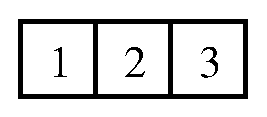
\includegraphics[width=1.5cm,height=1.5cm,keepaspectratio]
 {d3_s.eps}}  
\qquad\qquad
\raisebox{-0.6cm}{
 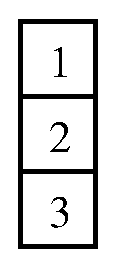
\includegraphics[width=1.5cm,height=1.5cm,keepaspectratio]
 {d3_a.eps}}  
\qquad\qquad
\raisebox{-0.35cm}{
 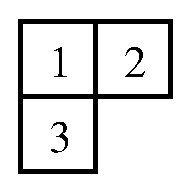
\includegraphics[width=1.0cm,keepaspectratio]
 {d3_t1.eps}} 
\qquad\qquad
\raisebox{-0.35cm}{
 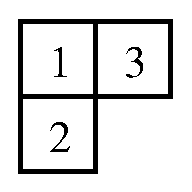
\includegraphics[width=1.0cm,keepaspectratio]
 {d3_t2.eps}}
\end{equation}

	The first diagram corresponds to an absolutely 
	symmetric component of the tensor:
\[
\raisebox{-0.1cm}{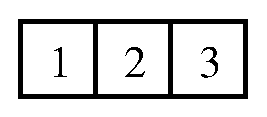
\includegraphics[width=1.5cm,height=1.5cm,keepaspectratio]
 {d3_s.eps}}
	~~\longrightarrow~~
	S^{\mu\nu\rho} ~=~ T^{(\mu\nu\rho)} ~=~
	T^{\mu\nu\rho} ~+~ 	T^{\nu\rho\mu} ~+~	T^{\rho\mu\nu} 
 ~+~	T^{\mu\rho\nu} ~+~ 	T^{\rho\nu\mu} ~+~	T^{\nu\mu\rho}~.
\]
	The second diagram is the absolutely antisymmetric component:
\[
\raisebox{-0.7cm}{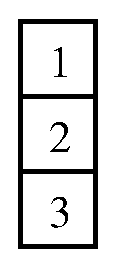
\includegraphics[width=1.5cm,height=1.5cm,keepaspectratio]
 {d3_a.eps}}
	~~\longrightarrow~~
	A^{\mu\nu\rho} ~=~ T^{[\mu\nu\rho]} ~=~
	T^{\mu\nu\rho} ~+~ 	T^{\nu\rho\mu} ~+~	T^{\rho\mu\nu} 
 ~-~	T^{\mu\rho\nu} ~-~ 	T^{\rho\nu\mu} ~-~	T^{\nu\mu\rho}~.
\]
	The two ``corner'' diagrams generate, correspondingly,
\[
\raisebox{-0.4cm}{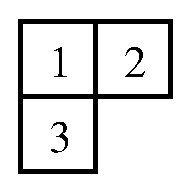
\includegraphics[width=1.0cm,height=1.0cm,keepaspectratio]
 {d3_t1.eps}}
	~~~~\longrightarrow~~~~
	T_1^{\mu\nu\rho} ~=~
	T^{\mu\nu\rho} ~-~ T^{\rho\nu\mu} ~+~ T^{\nu\mu\rho}
	~-~  T^{\rho\mu\nu}~,
\]
	and
\[
\raisebox{-0.4cm}{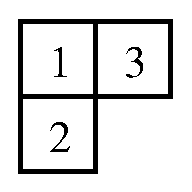
\includegraphics[width=1.0cm,height=1.0cm,keepaspectratio]
 {d3_t2.eps}}
	~~~~\longrightarrow~~~~
	T_2^{\mu\nu\rho} ~=~
	T^{\mu\nu\rho} ~-~ T^{\nu\mu\rho} ~+~ T^{\rho\nu\mu}
	~-~  T^{\nu\rho\mu}~.
\]
	To provide a slightly more complicated example of applying
	the (anti)symmetrization rules we demonstrate
	a diagram corresponding to an irreducible component of a 
	four-tensor:
\[
\raisebox{-0.6cm}{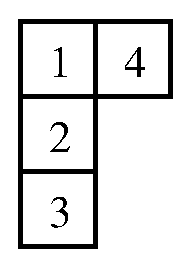
\includegraphics[width=1.5cm,height=1.5cm,keepaspectratio]
 {d4_sample.eps}}
	~~~~\longrightarrow~~~~
	T^{[\mu\nu\rho]\lambda} ~+~ T^{[\lambda\nu\rho]\mu}~.
\]

	All four components of \eqref{rank3_diags} 
	(weighed by appropriate coefficients) sum into
	the original tensor $ T^{\mu\nu\rho} $:
\[
	T^{\mu\nu\rho} ~=~
	\frac{1}{3!}\, \left\lgroup S^{\mu\nu\rho} ~+~
				 A^{\mu\nu\rho} ~+~
				 2 T_1^{\mu\nu\rho} ~+
				 2 T_2^{\mu\nu\rho} \right\rgroup~.
\]
	
	The last step to perform is subtract from each component
	all traces obtained by contraction of any two indices which
	are not antisymmetrized (contraction of antisymmetrized indices is
	trivial).
	The solution can be sought by means of a tensor of a rank
	$ r - 2 $:
\begin{equation}
\label{subtr_traces}
	T_{i\;{\rm (irr)}}^{\mu\nu\rho\lambda...} ~=~
	T_i^{\mu\nu\rho\lambda...}  ~-~  a^{\rho\lambda...}g^{\mu\nu} 
				  ~+~  a^{\rho\mu...}g^{\lambda\nu} ~+~ ...~,
\end{equation}
	where $ T_i^{\mu\nu\rho\lambda...} $ is the $ i $-the component
	obtained from the corresponding Young tableau.
	The traces part in the r.h.s. of \eqref{subtr_traces} should 
	possess the same symmetries as $ T_i^{\mu\nu\rho\lambda...} $
	so as to promote these symmetries to the l.h.s.
	Contracting any two indices in equation \eqref{subtr_traces} and
	requiring the result to vanish one can obtain the explicit expression
	for the trace $ a^{\rho\lambda..} $.


	

	
	
\end{document}
